% !TeX encoding = UTF-8
% !TeX program = xelatex
\PassOptionsToPackage{table}{xcolor}
\documentclass[UTF8,zihao=5,oneside,openany,fontset=fandol]{ctexbook}

\usepackage{graphicx,amsmath,amssymb,caption}
\newcommand{\setbaselineskip}[1]{\setlength{\baselineskip}{#1}}
% ===================== 参考文献 =====================
\usepackage[backend=biber,style=gb7714-2015]{biblatex}
\renewcommand{\bibfont}{\zihao{-5}\setbaselineskip{14bp}}
\setlength{\bibitemsep}{2bp plus 1pt}
\addbibresource{refs.bib}

% ===================== 配色 =====================
\usepackage{xcolor}
\definecolor{accent}{HTML}{1F4E8C}
\definecolor{accentlight}{HTML}{E8EEF6}
\definecolor{rowtint}{HTML}{F5F7FA}
\definecolor{inkmuted}{HTML}{55606E}
% 四段链路的固定配色，图与表一致
\definecolor{segbus}{HTML}{1F5FA8}
\definecolor{segrect}{HTML}{C8461E}
\definecolor{seghb}{HTML}{1E8A6E}
\definecolor{segpl}{HTML}{7A4FB0}

% ===================== 章节版式 =====================
\ctexset{
  chapter = {
    format     = \raggedright\heiti\zihao{3}\color{accent},
    nameformat = {},
    name       = {},
    number     = \arabic{chapter},
    aftername  = \hspace{0.8em},
    beforeskip = 0pt,
    afterskip  = 10bp,
    fixskip    = true,
  },
  section = {
    format    = \raggedright\heiti\zihao{-4}\color{accent},
    beforeskip= 10bp plus 2bp minus 1bp,
    afterskip = 4bp,
    aftername = \hspace{0.6em},
  },
  subsection = {
    format    = \raggedright\heiti\zihao{5},
    beforeskip= 6bp plus 1bp,
    afterskip = 2bp,
    aftername = \hspace{0.5em},
  },
}

% ===================== 版心 =====================
\usepackage{geometry}
\geometry{a4paper, top=23mm, bottom=20mm, left=22mm, right=22mm, headheight=21pt, headsep=6mm, footskip=8mm}
\setlength{\parskip}{0pt plus 1pt}

% ===================== 页眉页脚 =====================
\usepackage{fancyhdr}
\fancypagestyle{reportbody}{%
  \fancyhf{}%
  \fancyhead[L]{\small\color{inkmuted}托卡马克电源系统全链路仿真与校核}%
  \fancyhead[R]{\small\color{inkmuted}GKC3-Simulink 技术报告}%
  \fancyfoot[C]{\small\color{inkmuted}\thepage}%
  \renewcommand{\headrulewidth}{0.4pt}%
  \renewcommand{\headrule}{\hbox to\headwidth{\color{accent!35}\leaders\hrule height \headrulewidth\hfill}}%
  \renewcommand{\footrulewidth}{0pt}%
}

% ===================== 图 =====================
\graphicspath{{figures/}}
\DeclareGraphicsExtensions{.pdf,.png,.jpg}
\captionsetup{font=small, labelfont={bf,color=accent}, textfont=md, labelsep=quad, skip=3pt, justification=centering, singlelinecheck=true}
\captionsetup[table]{skip=4pt, position=top}
\setlength{\textfloatsep}{8pt plus 2pt minus 2pt}
\setlength{\floatsep}{7pt plus 2pt minus 2pt}
\setlength{\intextsep}{7pt plus 2pt minus 2pt}
\setcounter{topnumber}{3}
\setcounter{bottomnumber}{2}
\setcounter{totalnumber}{4}
\renewcommand{\topfraction}{0.92}
\renewcommand{\bottomfraction}{0.8}
\renewcommand{\textfraction}{0.08}
\renewcommand{\floatpagefraction}{0.8}
\usepackage{float}
\newcommand{\twofig}[4]{%
\begin{figure}[tbp]\centering
\includegraphics[width=0.8\linewidth,height=84mm,keepaspectratio]{#1}\\[0pt]{\small (a)}\\[2pt]
\includegraphics[width=0.8\linewidth,height=84mm,keepaspectratio]{#2}\\[0pt]{\small (b)}
\caption{#3}\label{#4}
\end{figure}}
% 模型视图分辨率足够，并排放置
\newcommand{\sidefig}[4]{%
\begin{figure}[tbp]\centering
\begin{minipage}[t]{0.49\linewidth}\centering\vspace{0pt}\includegraphics[width=\linewidth,height=58mm,keepaspectratio]{#1}\\[0pt]{\small (a)}\end{minipage}\hfill
\begin{minipage}[t]{0.49\linewidth}\centering\vspace{0pt}\includegraphics[width=\linewidth,height=58mm,keepaspectratio]{#2}\\[0pt]{\small (b)}\end{minipage}
\caption{#3}\label{#4}
\end{figure}}
\usepackage{placeins}
\makeatletter
\setlength{\@fptop}{0pt}
\setlength{\@fpsep}{8pt}
\setlength{\@fpbot}{0pt plus 1fil}
\makeatother

% ===================== 表 =====================
\usepackage{array,booktabs,tabularx,makecell,multirow,longtable}
\setlength{\aboverulesep}{0pt}
\setlength{\belowrulesep}{0pt}
\setlength{\heavyrulewidth}{0.9pt}
\setlength{\lightrulewidth}{0.45pt}
\arrayrulecolor{accent}
\newcommand{\tablefont}{\small\setlength{\extrarowheight}{0pt}\renewcommand{\arraystretch}{1.16}}
% 浅色表头与隔行底色
\newcommand{\headrow}{\rowcolor{accentlight}}
\newcommand{\zebra}{\rowcolors{1}{}{rowtint}}
\newcolumntype{L}{>{\raggedright\arraybackslash}X}
\newcolumntype{R}{>{\raggedleft\arraybackslash}X}
\newcolumntype{P}[1]{>{\raggedright\arraybackslash}p{#1}}
\newcolumntype{C}{>{\centering\arraybackslash}X}
\newenvironment{dtable}[2]{%
  \begin{table}[#1]\centering\tablefont\zebra\caption{#2}%
}{\end{table}}

% ===================== 正文小结框 =====================
\usepackage[most]{tcolorbox}
\newtcolorbox{keybox}{enhanced, breakable=false, colback=accentlight!55, colframe=accentlight!55,
  boxrule=0pt, arc=1.5pt, left=8pt, right=8pt, top=5pt, bottom=5pt, before skip=8pt, after skip=8pt,
  borderline west={2pt}{0pt}{accent}, fontupper=\small}

% ===================== 数学与单位 =====================
\usepackage{siunitx}
\sisetup{per-mode=symbol, detect-all=false, group-minimum-digits=5}
\providecommand{\dd}{\mathop{}\!\mathrm{d}}
\newcommand{\sub}[1]{_{\mathrm{#1}}}

% ===================== 绘图 =====================
\usepackage{tikz}
\usetikzlibrary{arrows.meta, positioning, fit, calc, backgrounds}
\usepackage[european resistors, american inductors]{circuitikz}

% ===================== 代码 =====================
\usepackage{listings}
\lstdefinestyle{repro}{%
  basicstyle=\ttfamily\footnotesize, columns=flexible, keepspaces=true, breaklines=true,
  backgroundcolor=\color{rowtint}, frame=leftline, rulecolor=\color{accent}, framerule=1.5pt,
  xleftmargin=1em, framexleftmargin=0.8em, aboveskip=6pt, belowskip=6pt,
  commentstyle=\color{inkmuted}, showstringspaces=false, upquote=true, extendedchars=false}
\lstnewenvironment{codeblock}[1][]{\lstset{style=repro,#1}}{}

% ===================== 超链接 =====================
\usepackage{hyperref}
\hypersetup{colorlinks=true, linkcolor=accent, citecolor=accent, urlcolor=accent,
  pdftitle={托卡马克电源系统全链路仿真与校核}, pdfauthor={GKC3-Simulink contributors}}
\urlstyle{tt}
\newcommand{\repourl}{https://github.com/KiloxGo/GKC3-Simulink}

% 正文行距
\AtBeginDocument{\setbaselineskip{17bp}}

% Allow long technical labels to wrap without changing report content.
\setlength{\emergencystretch}{3em}

\newenvironment{nomenclature}{\chapter*{主要符号}}{}
\NewDocumentEnvironment{abstract}{O{zh}}{\chapter*{\ifstrequal{#1}{en}{Abstract}{摘要}}}{}


\begin{document}

\hypersetup{pageanchor=false}
\begin{titlepage}
\centering
\vspace*{25mm}
{\color{accent}\sffamily\Large GKC3-Simulink\par}
\vspace{18mm}
{\heiti\Huge 托卡马克电源系统\par}
\vspace{5mm}
{\heiti\Huge 全链路仿真与校核\par}
\vspace{12mm}
{\Large Full-Chain Simulation and Verification\\of a Tokamak Power Supply System\par}
\vspace{16mm}
{\large 公开技术报告 · Public technical report\par}
\vfill
{\large GKC3-Simulink contributors\par}
\vspace{5mm}
\url{\repourl}\par
\vspace{8mm}
{\large 2026 年 11 月\par}
\end{titlepage}
\frontmatter
\hypersetup{pageanchor=true}
\pagestyle{plain}
% !TEX root = ../main.tex

\begin{abstract}[zh]
托卡马克的磁体与等离子体供电可以看作一条从交流电网到线圈的功率链。本报告整合课程的仿真工作：10~kV 母线下垂调压、CS 线圈 1.5~kV 整流供电、H 桥电流环、互感耦合可变等离子体负载，以及把这些环节接入同一电气网络的整机联合仿真。全部模型基于 MATLAB/Simulink R2026a 与 Simscape Electrical 搭建，校核采用与控制器设计无关的解析式、外部基准和守恒量。

分段结果为：母线六个工况与独立相量解的偏差不超过 $7.8\times10^{-5}$~pu；整流供电 460~s 全过程的 CS 电流峰值为 39.746~kA、输入功率峰值为 59.619~MW，八个关键时刻的电流与 ODE 基准最大相差 0.247\%；H 桥五段给定的稳态误差为 0.68--1.77~A，修正死区实现后全部换相间隔为 2~$\mu$s，无桥臂直通。整机模型以 1~$\mu$s 步长连续运行 30~s，平台段母线均值 2199.98~V，等离子体电流均值 9999.28~A，退磁时向交流侧净回馈 0.559~MJ。另一套晶闸管整流接口的联合模型给出了一致的负载侧结果，线圈侧能量相差 0.015\%。

横向比较表明，约 1~MW 的联合运行负载对 100~MVA 母线几乎没有影响，而实验一 59.6~MW 的峰值负载需要 1.46~pu 的内部电势，超出 1.15~pu 限幅，短路容量需提高到约 270~MVA 以上才能满足。

\vspace{0.5em}
\noindent\textbf{项目仓库：}\url{\repourl}
\vspace{0.3em}
\end{abstract}

\begin{abstract}[en]
The supply of a tokamak's magnets and plasma forms a power chain from the AC grid to the coils. This report consolidates the simulation work of the course: droop voltage regulation of a 10~kV bus, the 1.5~kV rectifier feeding the central solenoid (CS), an H-bridge current loop, a mutually coupled variable plasma load, and an integrated co-simulation that places these stages in one electrical network. All models are built with MATLAB/Simulink R2026a and Simscape Electrical, and are verified against analytic relations, external baselines and conserved quantities that are independent of the controller design.

Segment results: the six bus cases differ from an independent phasor solution by at most $7.8\times10^{-5}$~pu; the 460~s rectifier run reaches a CS current of 39.746~kA and an input power of 59.619~MW, with a maximum current deviation of 0.247\% from the ODE baseline at eight key instants; the H-bridge shows steady-state errors of 0.68--1.77~A over five reference segments, and after correcting the dead-time logic every commutation gap is 2~$\mu$s with no shoot-through. The integrated model runs continuously for 30~s at a 1~$\mu$s step: on the plateau the mean DC bus voltage is 2199.98~V and the mean plasma current is 9999.28~A, and demagnetization returns a net 0.559~MJ to the AC side. A second co-simulation with a thyristor rectifier interface gives consistent load-side results, with coil energies differing by 0.015\%.

Comparison across stages shows that the joint load of about 1~MW barely affects the 100~MVA bus, whereas the 59.6~MW peak of the rectifier experiment would require an internal EMF of 1.46~pu, beyond the 1.15~pu limit; the short-circuit capacity must exceed about 270~MVA.

\vspace{0.5em}
\noindent\textbf{Repository:} \url{\repourl}
\vspace{0.3em}
\end{abstract}

\hypersetup{linkcolor=black}
\tableofcontents
\hypersetup{linkcolor=accent}
% 符号表接排在目录之后，不单独占页
\ctexset{chapter/break={\par\addvspace{14bp}}}
% !TEX root = ../main.tex

\begin{nomenclature}
\small\renewcommand{\arraystretch}{1.12}
\begin{longtable}{P{0.26\linewidth}P{0.68\linewidth}}
\toprule
\rowcolor{accentlight} 符号 & 含义 \\
\midrule\addlinespace[2pt]
\endhead
\bottomrule
\endfoot
$E$，$E\sub{req}$ & 等值电源内部电势及维持给定工况所需的内部电势（标幺） \\
$Z_g$，$R_g$，$X_g$，$L_g$ & 电网等值阻抗及其电阻、电抗、电感 \\
$S\sub{sc}$，SCR & 短路容量与短路比 \\
$v\sub{pu}$，$p\sub{pu}$，$q\sub{pu}$ & 母线电压、有功、无功的瞬时标幺值 \\
$v\sub{f}$，$q\sub{f}$，$v\sub{ref}$ & 一阶滤波后的电压、无功及下垂电压目标 \\
$\alpha$ & 晶闸管触发角 \\
$U_d$，$U\sub{dc}$，$V\sub{dc}$ & 整流平均电压、直流母线电压 \\
$R\sub{eq}$，$L\sub{eq}$ & CS 端口的等效电阻、等效电感 \\
$i\sub{CS}$，$B\sub{CS}$，$E\sub{mag}$ & CS 电流、工程磁场与磁场储能 \\
$m\sub{H}$，$t_d$，$T_s$ & H 桥调制比、死区时间、载波周期 \\
$K_p$，$K_i$，$\omega_c$ & PI 比例、积分系数与穿越角频率 \\
$i\sub{cs}$，$i\sub{p}$，$i\sub{m}$ & 原边线圈电流、等离子体电流、励磁电流 \\
$\psi$，$k_\psi$ & 互感磁链、退磁比例系数 \\
$R\sub{p}$，$L\sub{p}$ & 等离子体回路的可变电阻、可变电感 \\
$L_1$，$L_2$，$k$，$L_\sigma$ & 互感两绕组自感、耦合系数、短路电感 \\
$C\sub{dc}$，$R\sub{br}$，$R\sub{bleed}$ & 直流母线电容、制动电阻、泄放电阻 \\
\end{longtable}
\end{nomenclature}


\mainmatter
\pagestyle{reportbody}
% 正文各章连续排版，浮动体不跨章
\ctexset{chapter/break={\FloatBarrier\par\addvspace{14bp}}}
% !TEX root = ../main.tex

\chapter{绪论}
\label{chap:intro}

\section{研究背景}

托卡马克依靠中央螺线管（CS）的电流变化在等离子体中感应出环向电流，一次放电要经历预磁化、击穿、升流、平顶和降流几个阶段\cite{wesson2011tokamaks}。对供电系统而言，这意味着一条从交流电网到线圈的功率链：电网提供有功和无功，变压器和可控整流器产生可调直流电压，变流器在毫秒尺度上控制线圈电流，负载参数则随放电阶段变化。

课程的分项实验各取这条链上的一节：实验一研究 CS 线圈的 1.5~kV 整流供电\cite{guide-cs}，实验二研究 10~kV 母线的下垂调压\cite{guide-droop}，实验三研究 H 桥电流环\cite{guide-hbridge}，实验四把 H 桥的负载换成互感耦合的可变等离子体负载\cite{guide-plasma}。这些模型的源假设各不相同：实验一用理想 10~kV 电源，实验二用 100~MVA 的等值电网，实验三、四用 2200~V 理想直流母线。

本报告把这些工作整合为一条完整的链路（图~\ref{fig:chain}），分三个层次展开：第 \ref{chap:bus}--\ref{chap:plasma} 章按功率流向逐段给出建模与校核；第 \ref{chap:joint} 章去掉各段之间的独立电源，把全部环节接入同一电气网络做联合仿真；第 \ref{chap:analysis} 章横向比较各段的量级与时间尺度，并定量回答分段模型无法回答的接口问题。

\begin{figure}[htbp]
\centering
\makebox[\linewidth][c]{\begin{tikzpicture}[font=\footnotesize, >={Latex[length=1.6mm]},
  block/.style={draw=#1, fill=#1!8, rounded corners=1.5pt, line width=0.6pt, align=center,
                minimum width=15.6mm, minimum height=11mm, inner sep=1pt},
  flow/.style={->, line width=0.7pt, color=black!70},
  seglabel/.style={font=\footnotesize\bfseries, text=#1},
  note/.style={font=\scriptsize, text=inkmuted, align=center}]
\node[block=segbus] (src) at (0,0) {受控\\三相源};
\node[block=segbus] (zg)  at (1.98,0) {电网阻抗\\$Z_g$};
\node[block=segrect] (tr)  at (3.96,0) {变压器\\10/1.2~kV};
\node[block=segrect] (rec) at (5.94,0) {六脉波\\全控桥};
\node[block=segrect] (dc)  at (7.92,0) {平波电抗\\母线电容};
\node[block=seghb]  (hb)  at (9.90,0) {H 桥\\电流环};
\node[block=segpl]  (m)   at (11.88,0) {互感\\耦合};
\node[block=segpl]  (pl)  at (13.86,0) {$R\sub{p}(t)$\\$L\sub{p}(t)$};
\draw[flow] (src)--(zg);
\draw[flow] (zg)--(tr);
\draw[flow] (tr)--(rec);
\draw[flow] (rec)--(dc);
\draw[flow,<->] (dc)--(hb);
\draw[flow,<->] (hb)--(m);
\draw[flow,<->] (m)--(pl);
\node[block=inkmuted, minimum height=8mm, below=7mm of dc] (br) {制动 / 泄放};
\draw[flow] (dc)--(br);
\node[block=segbus, minimum height=8mm, below=7mm of $(src)!0.5!(zg)$, minimum width=28mm] (ctl) {$Q$--$V$ 下垂与电压 PI};
\draw[flow,dashed] (zg.south) -- (zg.south|-ctl.north);
\draw[flow,dashed] (src.south|-ctl.north) -- (src.south);
\node[seglabel=segbus, above=7.7mm of $(src)!0.5!(zg)$] (l1) {实验二};
\node[seglabel=segrect, above=2.2mm of rec] (l2) {实验一};
\node[seglabel=seghb, above=2.2mm of hb] (l3) {实验三};
\node[seglabel=segpl, above=7.7mm of $(m)!0.5!(pl)$] (l4) {实验四};
\draw[segbus, line width=1pt] ($(src.north west)+(0,1.5mm)$) -- ($(zg.north east)+(0,1.5mm)$);
\draw[segrect, line width=1pt] ($(tr.north west)+(0,1.5mm)$) -- ($(dc.north east)+(0,1.5mm)$);
\draw[seghb, line width=1pt] ($(hb.north west)+(0,1.5mm)$) -- ($(hb.north east)+(0,1.5mm)$);
\draw[segpl, line width=1pt] ($(m.north west)+(0,1.5mm)$) -- ($(pl.north east)+(0,1.5mm)$);
\node[note, below=7.5mm of $(m)!0.5!(pl)$, text width=36mm] {双向箭头：退磁时\\能量经 H 桥返回母线};
\end{tikzpicture}}
\caption{托卡马克供电链路与各实验的对应关系。第 \ref{chap:joint} 章的联合模型把这些环节接入同一电气网络。}
\label{fig:chain}
\end{figure}

\section{模型层次与主要结果}

表~\ref{tab:summary} 汇总了各项工作的结果及其校核依据。本报告的主要工作有三点：

\begin{itemize}
  \item 分段校核：四个模型统一在 R2026a 的 Simscape Electrical 上重建，每段都用独立于控制器的关系验收。
  \item 全链路联合：把各环节接入同一电气网络，在一次 30~s 连续运行中观察交流侧、直流母线、H 桥和等离子体负载，并用累计能量闭合功率账目；另用晶闸管整流接口的联合模型做交叉对照。
  \item 接口分析：用实验二的母线阻抗核算实验一的负载，得到这条母线所能承受的负载上限；把四段的时间尺度和“指令—实际”偏差放在同一口径下比较。
\end{itemize}

\begin{dtable}{htbp}{各项仿真工作的主要结果}
\label{tab:summary}
\begin{tabularx}{\linewidth}{P{0.2\linewidth}P{0.26\linewidth}P{0.2\linewidth}L}
\toprule
\headrow 环节 & 主要指标 & 结果 & 校核依据 \\
\midrule
10~kV 母线 & 默认工况母线电压 & 0.987803~pu & 相量解偏差 $2.8\times10^{-8}$~pu \\
CS 整流供电 & 电流峰值 / 输入功率峰值 & 39.746~kA / 59.619~MW & 八点 ODE 基准，电流差 $\le0.247\%$ \\
H 桥电流环 & 五段稳态误差 & 0.68--1.77~A & 回路方程稳态残差 2.85~V（均方根） \\
可变等离子体负载 & 平台段电流 / 功率 & 10.01~kA / 1.001~MW & 磁链两条路径残差约 0.011~Wb \\
整机联合 & 平台段母线 / 等离子体电流 & 2199.98~V / 9999.28~A & 接口能量闭合，退磁净回馈 0.559~MJ \\
晶闸管接口对照 & 平台段母线 / 等离子体电流 & 1499.81~V / 10.0000~kA & 直流能量残差 0.00318\% \\
\bottomrule
\end{tabularx}
\end{dtable}

% !TEX root = ../main.tex

\chapter{建模环境与校核方法}
\label{chap:method}

\section{建模平台}

全部模型在 MATLAB/Simulink R2026a 中搭建，电气部分采用 Simscape Electrical，控制部分采用 Simulink 基础模块。课程指导书基于 Specialized Power Systems 库编写，而 R2026a 已不再提供该库，因此各模型在保持拓扑、参数和时序不变的前提下，电气部分改用 Simscape 元件实现：IGBT 和二极管采用理想开关半导体模型，通态电阻 20~$\mu\Omega$、正向压降 2~V，与指导书一致；物理网络采用局部后向欧拉法离散求解。

Simscape 半导体模型为分段线性模型，不含开关暂态、拖尾电流和反向恢复过程，因此本报告的分析和结论限于开关周期及更长的时间尺度。

\section{三类独立校核}

用控制器内部的中间量证明控制器正确，并不能提供新的信息。各段模型采用三类与控制器设计无关的关系验收，见表~\ref{tab:checks}。

\begin{dtable}{htbp}{三类校核方法及其在各段的应用}
\label{tab:checks}
\begin{tabularx}{\linewidth}{P{0.13\linewidth}P{0.3\linewidth}L}
\toprule
\headrow 类别 & 含义 & 应用实例 \\
\midrule
解析式 & 只依赖拓扑和参数，不依赖 PI 参数 & 整流电压 $1.35U\sub{LL}\cos\alpha$，调制律 $\langle v\sub{AB}\rangle=U\sub{dc}m\sub{H}$，纹波估计 \\
外部基准 & 换一种算法得到的结果 & 实验一的 ODE 基准八点，实验二的稳态相量解，实验三的负载回路方程 \\
守恒量 & 能量和磁链的闭合关系 & 实验四磁链两条路径，联合模型的能量闭合与退磁能量链 \\
\bottomrule
\end{tabularx}
\end{dtable}

此外，53 项明确的课堂参数（电网阻抗、下垂系数、器件参数、PI 增益、PWM 时钟、死区常数、互感与查表数值等）已与指导书逐项核对，全部一致。这只是参数核对的结果，并不等于所有课程要求都已验收。

\section{求解设置}

各模型关心的现象相差很远，求解设置也各不相同（表~\ref{tab:solver}）。CS 整流的平均值模型用 0.01~s 步长跑完 460~s，整机模型则以 1~$\mu$s 定步长求解 30~s，共 3000 万步。第 \ref{chap:analysis} 章将进一步讨论时间尺度对建模方式的约束。

\begin{dtable}{htbp}{各模型的时间尺度与求解设置}
\label{tab:solver}
\begin{tabularx}{\linewidth}{P{0.2\linewidth}LP{0.15\linewidth}P{0.08\linewidth}P{0.12\linewidth}}
\toprule
\headrow 模型 & 要观察的现象 & 步长 & 时长 & 规模 \\
\midrule
CS 整流（平均值） & 磁体电流与储能的秒级变化 & 0.01~s（上限） & 460~s & 4.6 万点 \\
CS 整流（详细） & 换相与 300~Hz 纹波 & 50~$\mu$s & 0.5~s & 1 万步 \\
10~kV 母线 & 工频周期与下垂收敛 & 50~$\mu$s（上限） & 2~s & 4 万点 \\
H 桥 & 2~kHz 载波与 2~$\mu$s 死区 & 1~$\mu$s & 0.42~s & 42 万步 \\
等离子体负载 & 开关周期与 30~s 磁链变化 & 10~$\mu$s & 30~s & 300 万步 \\
整机联合 & 交流侧到负载的完整耦合 & 1~$\mu$s & 30~s & 3000 万步 \\
晶闸管接口对照 & 换相、母线与制动的耦合 & 2~$\mu$s & 30~s & 1500 万步 \\
\bottomrule
\end{tabularx}
\end{dtable}

% !TEX root = ../main.tex

\chapter{交流母线：10~kV 下垂调压}
\label{chap:bus}

\section{拓扑与阻抗}

实验二的对象是一台可调内部电势 $E$ 经有限阻抗向 10~kV 母线供电的三相电源，功率通路和控制结构如图~\ref{fig:droop-model} 所示。母线测点 M1 位于阻抗之后：若放在阻抗之前，控制器看到的只是自身的指令，线路压降无法被补偿，下垂调压也失去物理意义。

电网短路容量 100~MVA、$X/R=5$，由 $|Z_g|=V_b^2/S\sub{sc}=1\ \Omega$ 得
\begin{equation}
R_g=\frac{1}{\sqrt{1+5^2}}=0.196116\ \Omega,\quad
X_g=5R_g=0.980581\ \Omega,\quad
L_g=\frac{X_g}{2\pi f}=3.121285\ \mathrm{mH}.
\label{eq:zg}
\end{equation}
短路容量只用于求阻抗，控制量的标幺化以 10~MVA 为功率基准。指导书未给测试变压器参数，主验证模型补充了一台 10~MVA、Yg/Yg、10:1 的理想化变压器，漏抗、励磁和饱和均关闭，默认二次侧每相 $R_2=X_2=0.2\ \Omega$，折算到一次侧为 $20+\mathrm{j}20\ \Omega$。

\begin{figure}[htbp]
\centering
\makebox[\linewidth][c]{\begin{tikzpicture}[font=\footnotesize, >={Latex[length=1.5mm]},
  pw/.style={draw=segbus, fill=segbus!8, rounded corners=1.5pt, line width=0.6pt, align=center, minimum width=19mm, minimum height=10mm, inner sep=1pt},
  ct/.style={draw=seghb, fill=seghb!8, rounded corners=1.5pt, line width=0.6pt, align=center, minimum width=19mm, minimum height=10mm, inner sep=1pt},
  flow/.style={->, line width=0.7pt, color=black!75},
  sig/.style={->, line width=0.6pt, dashed, color=black!60}]
\node[pw] (src) at (0,0) {受控三相源\\$E\angle\delta$};
\node[pw] (zg) at (2.72,0) {电网阻抗\\$R_g,\ L_g$};
\node[pw] (m1) at (5.44,0) {测点 M1\\10~kV 母线};
\node[pw] (tr) at (8.16,0) {变压器\\10:1};
\node[pw] (m2) at (10.88,0) {测点 M2};
\node[pw] (ld) at (13.6,0) {负载\\$R_2+\mathrm{j}X_2$};
\foreach \a/\b in {src/zg, zg/m1, m1/tr, tr/m2, m2/ld}{\draw[flow] (\a)--(\b);}
\node[ct] (meas) at (5.44,-1.9) {瞬时量计算\\$v\sub{pu},\ q\sub{pu}$};
\node[ct] (filt) at (2.72,-3.5) {一阶低通\\$\tau_V,\ \tau_Q$};
\node[ct] (dr) at (5.44,-3.5) {无功下垂\\系数 0.05};
\node[ct] (pi) at (8.16,-3.5) {PI 与限幅\\$K_p,\ K_i$};
\node[ct] (ed) at (10.88,-3.5) {内电势动态\\$\tau_E$};
\node[ct] (cmd) at (13.6,-3.5) {$E\in$\\$[0.85,1.15]$~pu};
\draw[sig] (m1)--(meas);
\draw[sig] (meas.west) -| (filt.north);
\draw[sig] (filt)--(dr);
\draw[sig] (dr)--(pi);
\draw[sig] (pi)--(ed);
\draw[sig] (ed)--(cmd);
\draw[sig] (cmd.south) |- ++(-6,-0.55) -| (0,-1.3) -- (src.south);
\end{tikzpicture}}
\caption{实验二的功率通路（上）与下垂调压控制（下）：母线测点位于电网阻抗之后，控制器调节阻抗之前的内部电势}
\label{fig:droop-model}
\end{figure}

\begin{figure}[htbp]
\centering
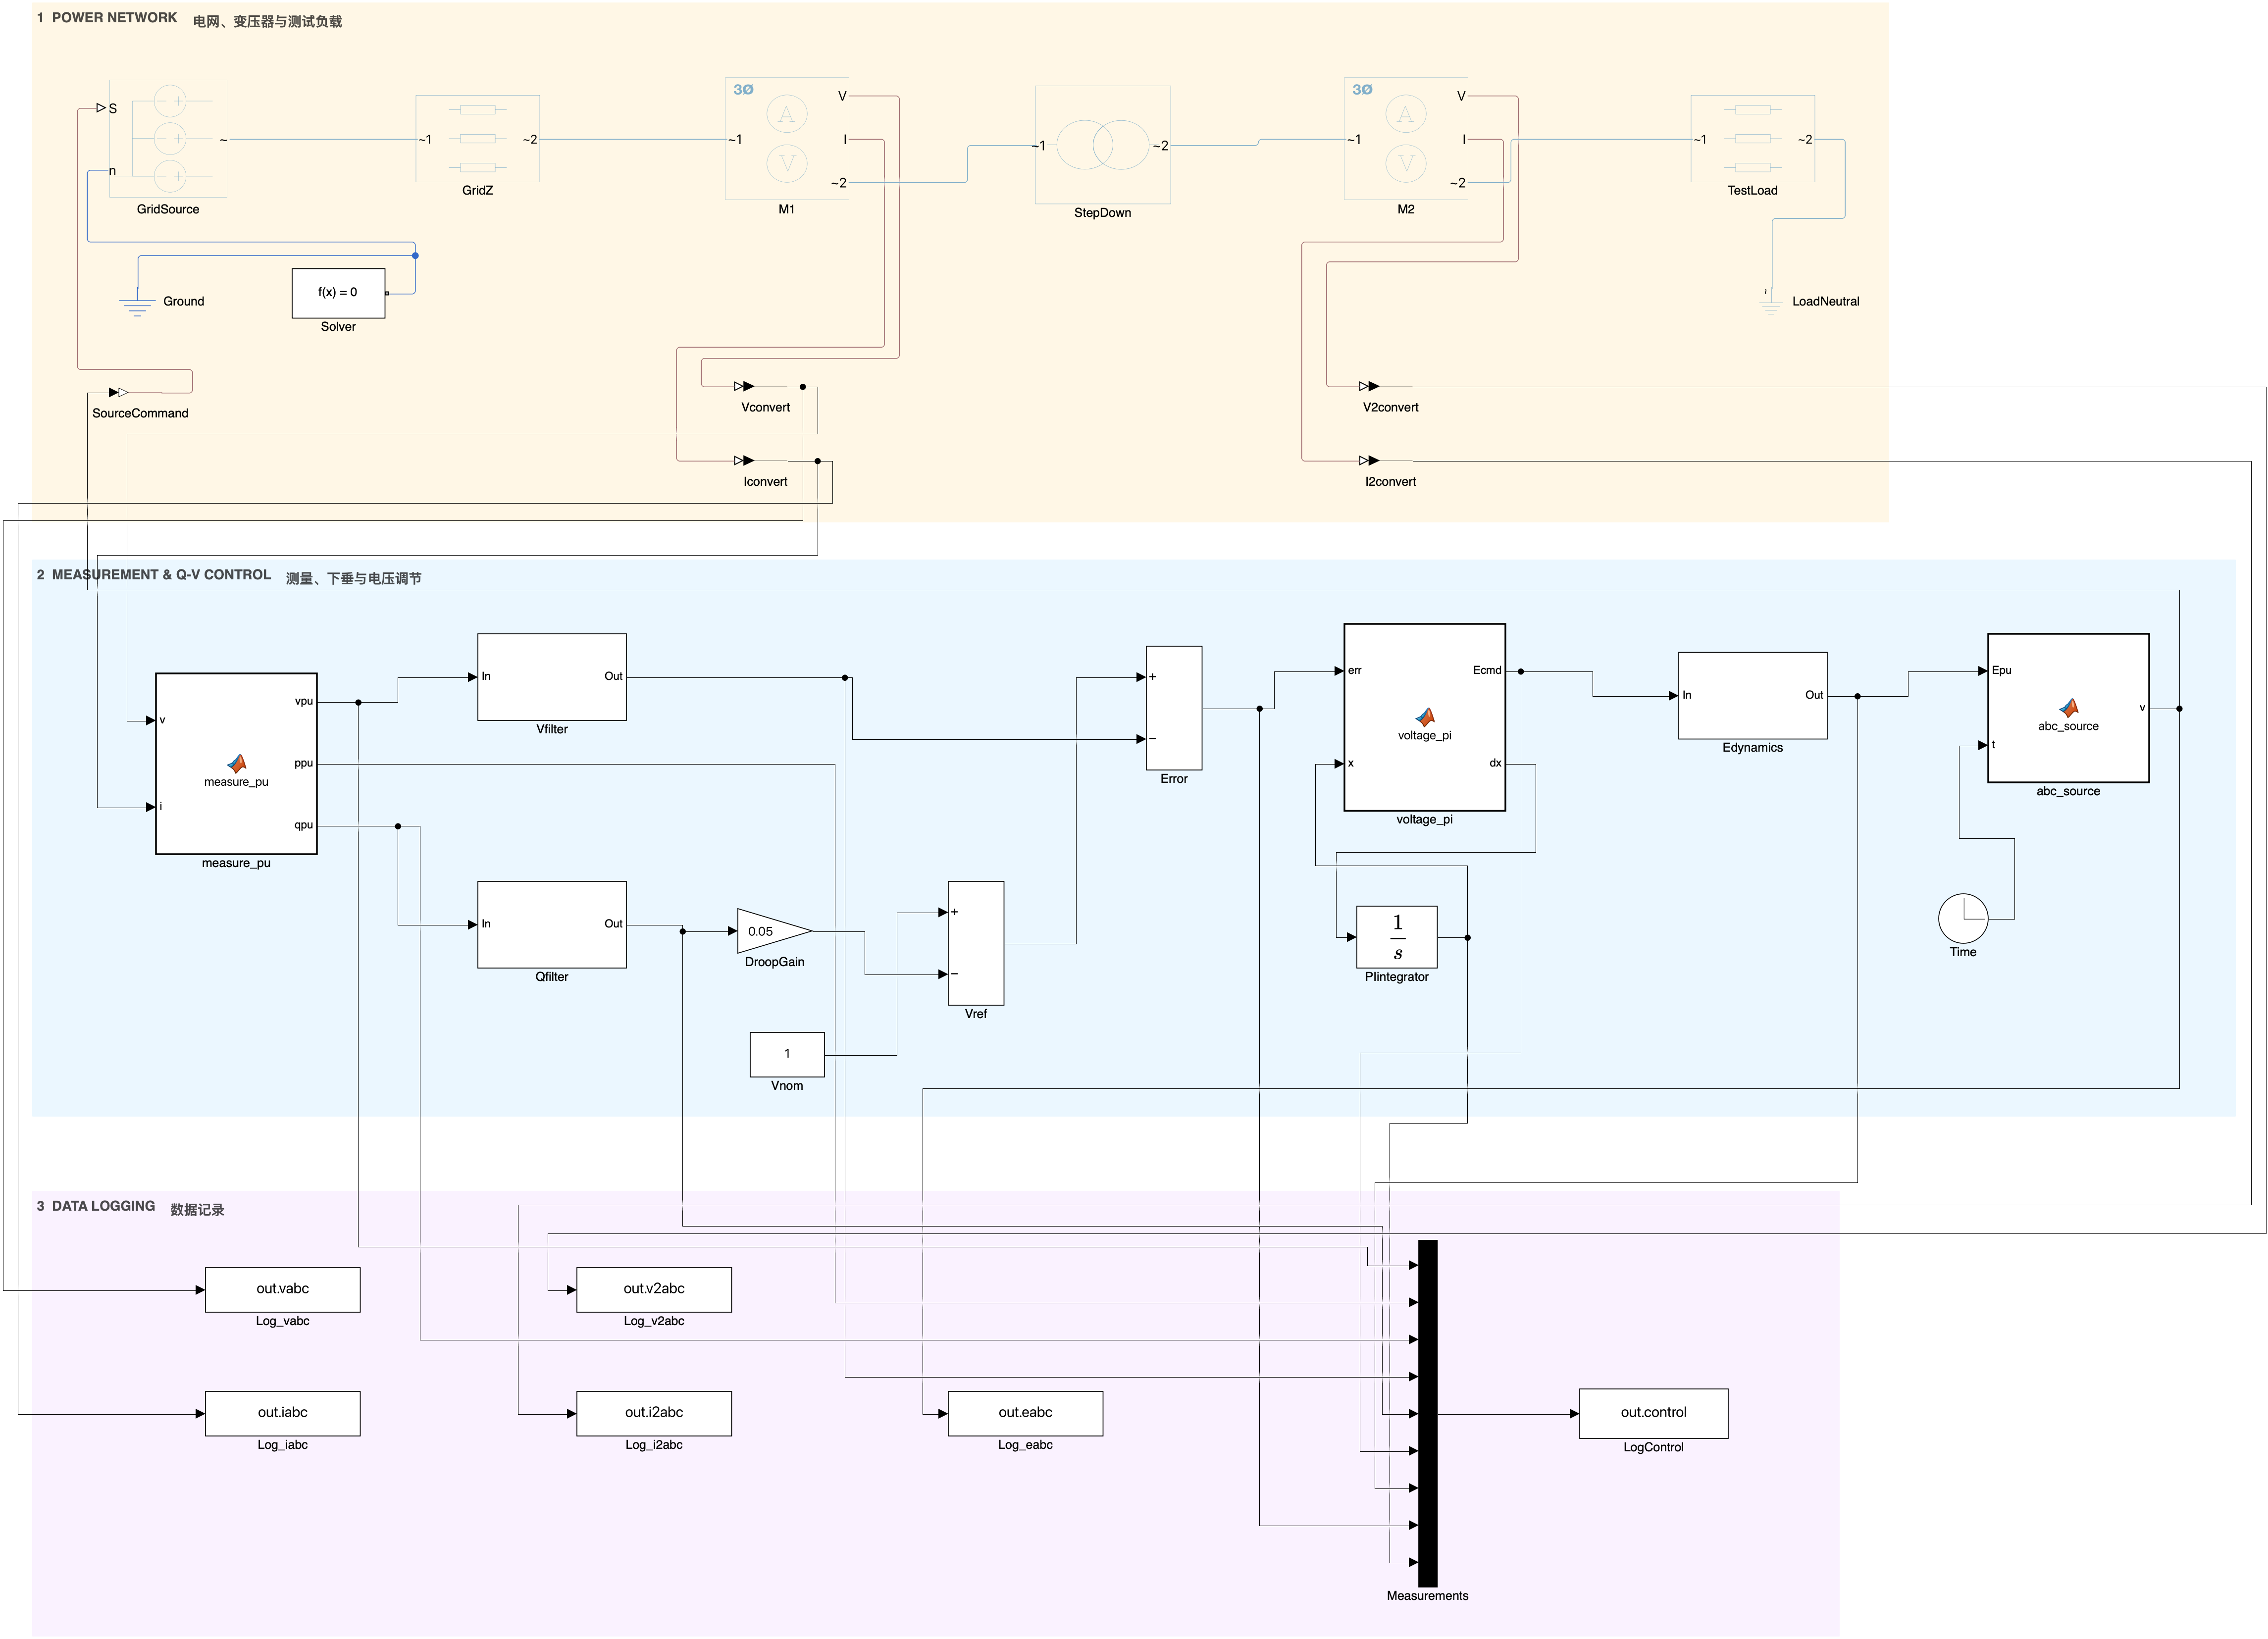
\includegraphics[width=0.62\linewidth]{native/model_droop.png}
\caption{实验二模型顶层（Simulink 原生视图）：电气网络、测量与下垂调压、数据记录三个分区}
\label{fig:droop-native}
\end{figure}

\section{测量与控制}

M1 输出三相瞬时电压和电流。取等幅值 Clarke 变换
\begin{equation}
v_\alpha=\frac{2}{3}\Bigl(v_a-\frac{v_b}{2}-\frac{v_c}{2}\Bigr),\qquad
v_\beta=\frac{\sqrt3}{3}(v_b-v_c),
\end{equation}
电流同理，并按瞬时功率理论\cite{akagi2007}计算标幺量：
\begin{equation}
v\sub{pu}=\frac{\sqrt{1.5(v_\alpha^2+v_\beta^2)}}{10^4},\quad
p\sub{pu}=\frac{v_ai_a+v_bi_b+v_ci_c}{10^7},\quad
q\sub{pu}=\frac{1.5(v_\beta i_\alpha-v_\alpha i_\beta)}{10^7}.
\label{eq:pq}
\end{equation}
平衡正弦条件下 $v\sub{pu}$ 即线电压有效值相对 10~kV 的标幺值，感性负载给出正无功。

电压、无功和内部电势各经一阶环节，时间常数为 $\tau_V=0.01$~s、$\tau_Q=0.02$~s、$\tau_E=0.05$~s。无功下垂给出电压目标\cite{kundur1994}
\begin{equation}
v\sub{ref}=1-0.05\,q\sub{f}.
\label{eq:droop}
\end{equation}
电压误差 $e=v\sub{ref}-v\sub{f}$ 送入 PI 控制器（$K_p=0.5$，$K_i=10\ \mathrm{s^{-1}}$），输出限幅后加在 1 上得到内部电势指令 $E\sub{cmd}\in[0.85,1.15]$~pu。抗饱和采用条件积分：控制器处于限幅且误差继续朝饱和方向时积分增量置零，误差反向后积分立即恢复。

限幅对象是阻抗之前的内部电势。轻中载时控制器可以抬高 $E$ 补偿 $Z_g$ 上的压降，$E$ 触及 1.15~pu 后母线电压就无法继续抬升。这一点是第 \ref{chap:analysis} 章接口核算的关键。

\section{独立相量解}

为避免仿真自证，另外写出不经过 Simulink 积分器的稳态相量解。令 $Z_t=Z_L+100(Z_2+r_w)$（$r_w$ 为微小绕组电阻），负载无功写成 $q\sub{pu}=cV\sub{pu}^2$，其中 $c=10\,\mathrm{Im}(Z_L)/|Z_t|^2$。未限幅时稳态同时满足式~\eqref{eq:droop}，解得
\begin{equation}
V\sub{pu}=\frac{2}{1+\sqrt{1+0.2c}},\qquad
E\sub{req}=V\sub{pu}\frac{|Z_g+Z_t|}{|Z_t|}.
\label{eq:phasor}
\end{equation}
若 $E\sub{req}>1.15$~pu，则把源电势固定在上限，再按电压分配重算母线电压。

\section{六个工况的结果}

图~\ref{fig:bus-response} 给出默认工况的启动过程和稳态三相波形。默认工况下母线先因 $Z_g$ 压降下降，无功经低通后逐渐建立，$v\sub{ref}$ 降到约 0.9878~pu，PI 同时把 $E$ 抬到 1.0170~pu，$v\sub{f}$ 与 $v\sub{ref}$ 重合，说明未限幅时闭环无差。末段 $V\sub{bus}=0.987803$~pu，而由 $Q/S_b=0.243938$ 计算的下垂目标为 0.9878031~pu，两者相差 $3.9\times10^{-12}$~pu。

三相波形在 1.94--2.00~s 内平衡、周期 20~ms。一次线电压有效值 9877.83~V，二次侧 987.783~V，比值 10.000；相邻相相位差为 $-120.00002^\circ$ 和 $-119.99998^\circ$，三相电压和的峰值为 $8.5\times10^{-8}$~V，没有共模偏置。

\twofig{native/bus_voltage_power.pdf}{native/bus_three_phase.pdf}{默认 RL 工况的 MATLAB 原生波形：(a) 启动段电压与功率，(b) 稳态三相相电压}{fig:bus-response}

\begin{figure}[htbp]
\centering
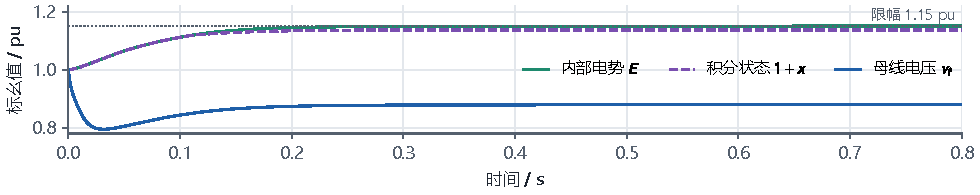
\includegraphics[width=\linewidth]{bus_saturation}
\caption{零积分初值重载工况：内部电势触及限幅后积分状态冻结，母线停在 0.8786~pu}
\label{fig:bus-sat}
\end{figure}

表~\ref{tab:bus-cases} 是六个工况的末段时间平均值。近空载和纯电阻工况 $Q\approx0$，目标为 1~pu，纯电阻工况为克服有功电流的线路压降把 $E$ 升到 1.011~pu。从默认 RL 到较强感性，$Q$ 由 2.44~Mvar 升到 3.85~Mvar，母线按下垂规律由 0.9878~pu 降到 0.9808~pu。

\begin{dtable}{htbp}{六个工况的稳态结果与独立相量解偏差}
\label{tab:bus-cases}
\begin{tabularx}{\linewidth}{LRRRRR}
\toprule
\headrow 工况 & $V\sub{bus}$ / pu & $P$ / MW & $Q$ / Mvar & $E$ / pu & $|\Delta V|$ / pu \\
\midrule
近空载 & 1.000000 & 0.00100 & 0.00000 & 1.000002 & $6.4\times10^{-8}$ \\
纯电阻 & 1.000000 & 4.99999 & 0.00000 & 1.010995 & $9.1\times10^{-8}$ \\
默认 RL & 0.987803 & 2.43934 & 2.43938 & 1.017047 & $2.8\times10^{-8}$ \\
较强感性 & 0.980762 & 1.92375 & 3.84754 & 1.023143 & $1.6\times10^{-7}$ \\
零初值重载 & 0.878646 & 19.30053 & 19.22465 & 1.150000 & $7.8\times10^{-5}$ \\
默认 RL 半步长 & 0.987803 & 2.43938 & 2.43938 & 1.017046 & $2.5\times10^{-9}$ \\
\bottomrule
\end{tabularx}
\end{dtable}

零初值重载是唯一撞限幅的工况（图~\ref{fig:bus-sat}）。负载折算到一次侧只有 $2+\mathrm{j}2\ \Omega$，稳态所需内部电势超过 1.15~pu。$E\sub{cmd}$ 在 0.110525~s 首次触及上限，此后 $E$ 按 $\tau_E$ 平滑跟随；积分状态涨到 0.137388~pu 后冻结。母线最终落在 0.878646~pu，比下垂目标 0.903877~pu 低 0.025230~pu，这一残余误差反映电源能力不足，与 PI 参数无关。

默认工况把最大步长由 $5\times10^{-5}$~s 减半后，母线末段均值只变化 $2.53\times10^{-8}$~pu，相量偏差由 $2.8\times10^{-8}$~pu 降到 $2.5\times10^{-9}$~pu，结果与步长无关。

100~MVA 短路容量与 2.44~MW 负载之比为 41，属于很强的母线，所以默认工况电压只下降 1.2\%。这一判断只对该负载成立，第 \ref{chap:analysis} 章将说明它不能外推到实验一的 59.6~MW。

% !TEX root = ../main.tex

\chapter{直流侧：CS 线圈的 1.5~kV 整流供电}
\label{chap:rect}

\section{电压变换与控制}

CS 线圈需要电压可调、电流很大的直流电源。实验一用 70~MVA、10/1.2~kV 的 $\Delta$/Y 变压器降压，六脉波全控桥整流后接时变 R-L 负载。连续电流下全控桥的平均输出为\cite{mohan2003}
\begin{equation}
V\sub{dc}=\frac{3\sqrt2}{\pi}U\sub{LL}\cos\alpha\approx1.35U\sub{LL}\cos\alpha.
\label{eq:rect}
\end{equation}
取 $U\sub{LL}=1.2$~kV、$V\sub{dc}=1.5$~kV，得初始触发角 $\alpha_0=\arccos[1500/(1.35\times1200)]=22.192^\circ$。短时仿真测得二次侧三个线电压有效值为 1199.37、1199.36、1199.22~V，最大相差 0.15~V，相序和变比正确。这一检查在接入整流桥和复杂负载之前完成，可以把电源接线问题与后级控制问题分开。

闭环控制器只看直流电压误差。式~\eqref{eq:rect} 在 $0^\circ<\alpha<90^\circ$ 内单调下降，$V\sub{dc}$ 偏低时减小 $\alpha$，反之增大。实现上以 $\alpha_0$ 作前馈工作点，PI 只补偿负载变化和模型误差，输出限制在 $5^\circ$--$80^\circ$。详细模型另加 10~ms 低通和积分限幅，避免 300~Hz 纹波直接驱动积分器。

全过程采用平均值模型：按式~\eqref{eq:rect} 产生直流电压并保留一阶变流器动态，省略器件级换相，以 0.01~s 步长跑完 460~s。六脉波详细模型只跑 0.5~s，用于验证式~\eqref{eq:rect} 背后的触发顺序和纹波机制。两层模型共用同一套负载参数和测量定义，慢动态指标和开关级波形可以直接对照。

\begin{figure}[htbp]
\centering
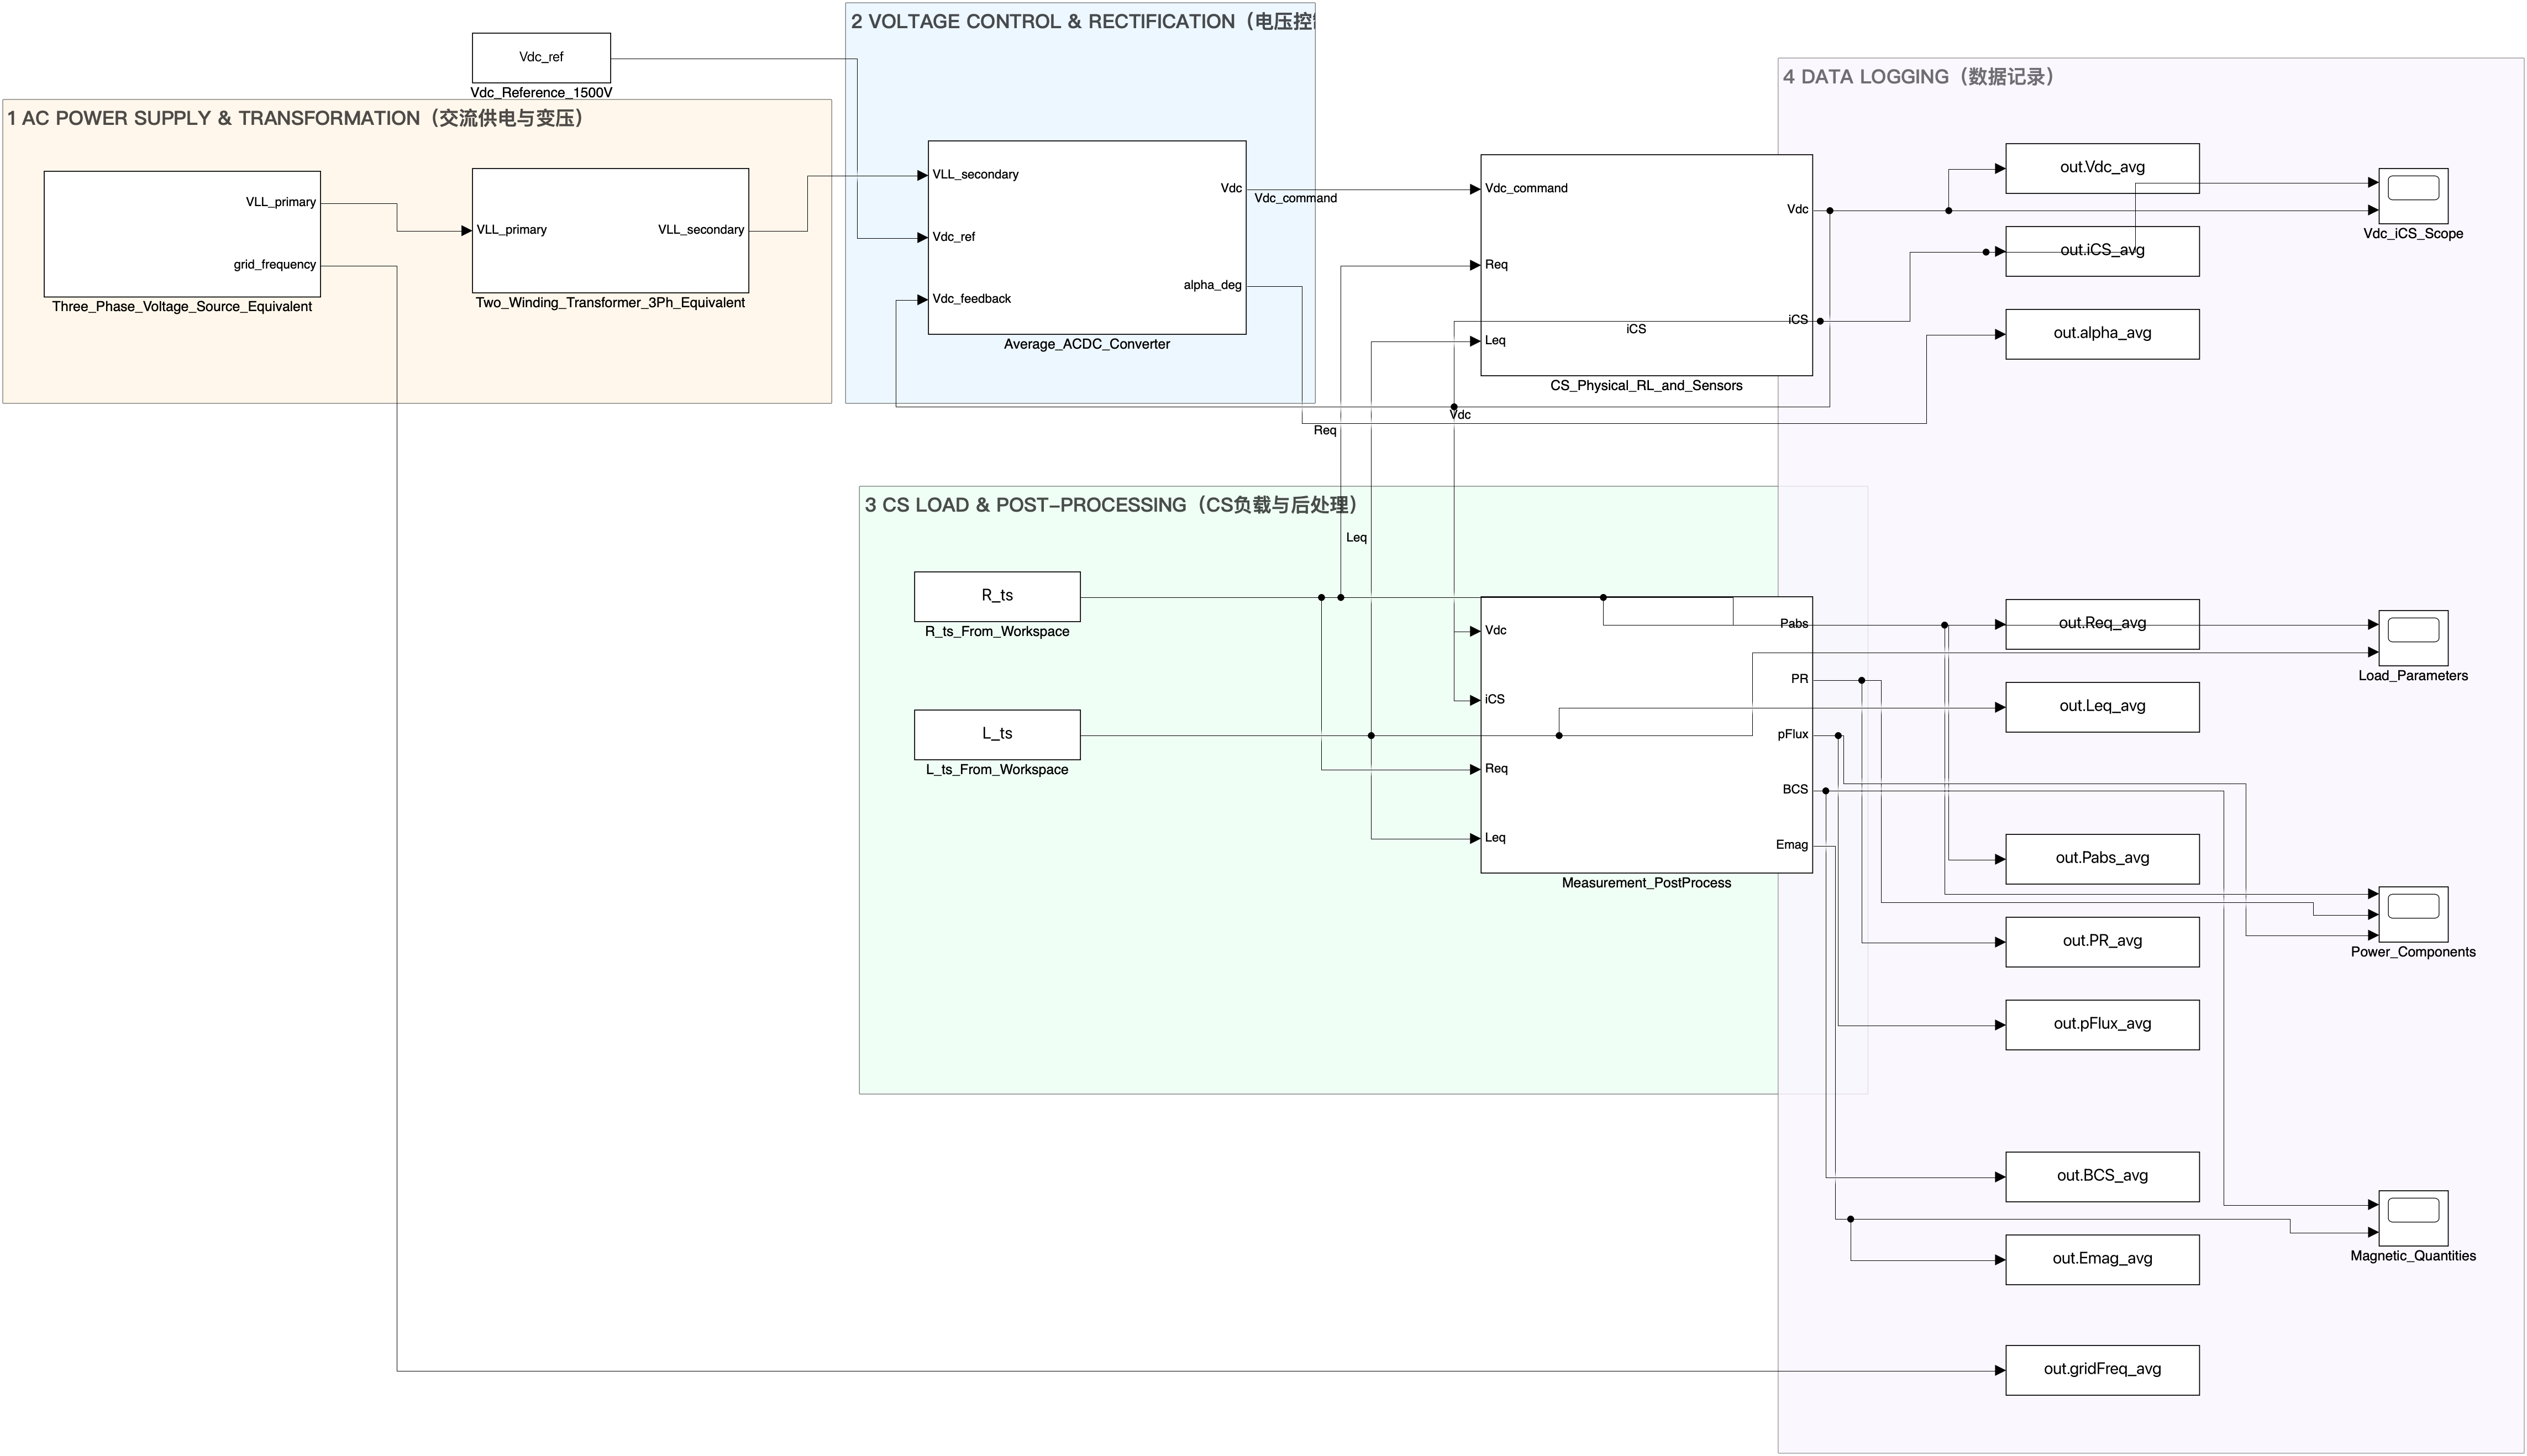
\includegraphics[width=0.66\linewidth]{native/model_cs.png}
\caption{实验一平均值模型顶层（Simulink 原生视图）：交流电源与变压、电压控制与整流、CS 负载与后处理、数据记录}
\label{fig:cs-native}
\end{figure}

\section{时变等效负载}

负载方程为
\begin{equation}
v\sub{CS}=R\sub{eq}(t)\,i\sub{CS}+\frac{\dd}{\dd t}\bigl[L\sub{eq}(t)\,i\sub{CS}\bigr].
\label{eq:cs-load}
\end{equation}
九个关键点（表~\ref{tab:cs-points}）在 0.01~s 网格上用 PCHIP 插值。选择 PCHIP 是因为它在关键点之间不产生过冲：$R\sub{eq}$ 在 12~s 附近由 0.6~$\Omega$ 降到 0.024~$\Omega$，普通样条的过冲会让电流曲线出现虚假拐点。这九个点描述的是整流器看到的等效端口，并非超导绕组本身的电阻或某一线圈的自感。Simscape 的 Variable Inductor 直接实现 $\dd(Li)/\dd t$，不需要再额外串联 $i\,\dd L/\dd t$ 电压源。

\begin{dtable}{htbp}{时变等效端口参数的九个关键点}
\label{tab:cs-points}
\begin{tabularx}{0.72\linewidth}{RRRL}
\toprule
\headrow $t$ / s & $R\sub{eq}$ / $\Omega$ & $L\sub{eq}$ / H & 阶段 \\
\midrule
0   & 0.35  & 1.10 & 预磁化 \\
5   & 0.80  & 1.08 & 击穿开始 \\
8   & 0.60  & 1.03 & 通道形成 \\
12  & 0.024 & 0.98 & 高导电形成 \\
45  & 0.024 & 0.95 & 爬升后段 \\
70  & 0.12  & 1.02 & 平顶开始 \\
335 & 0.12  & 1.00 & 平顶结束 \\
420 & 0.25  & 1.08 & 降流过程 \\
460 & 0.35  & 1.12 & 终止末段 \\
\bottomrule
\end{tabularx}
\end{dtable}

\section{全过程结果}

460~s 平均值模型的结果见图~\ref{fig:cs-overview}。直流电压全程稳定在 1.5~kV。电流可分三段：12~s 之前 1~H 量级的电感限制了电流变化率；12--45~s 电阻降到 0.024~$\Omega$，电源电压几乎全部用于建立磁链，电流快速爬升，在 50.262~s 达到峰值 39.746~kA；70~s 以后电阻回到 0.12~$\Omega$，电流朝 $1500/0.12=12.5$~kA 的平衡点衰减并形成平台，335~s 后电阻继续上升，电流降到 4.39~kA 结束。

\twofig{native/cs_voltage_current.pdf}{native/cs_power_field_energy.pdf}{平均值模型 460~s 的 MATLAB 原生波形：(a) 直流电压与 CS 电流，(b) 功率、工程磁场与磁场储能}{fig:cs-overview}

输入功率 $P\sub{abs}=v\sub{CS}i\sub{CS}$ 峰值为 59.619~MW，与电流峰值同时出现。磁场按 $B\sub{CS}=13i\sub{CS}/45000$ 换算，峰值 11.482~T。储能 $E\sub{mag}=\tfrac12L\sub{eq}i\sub{CS}^2$ 在 50.602~s 达到 0.7571~GJ，比电流峰值晚 0.34~s，原因是 $L\sub{eq}$ 此时仍在变化。

由式~\eqref{eq:cs-load} 可写出磁链相关功率及储能变化率：
\begin{equation}
p\sub{flux}=L\sub{eq}i\sub{CS}\frac{\dd i\sub{CS}}{\dd t}+i\sub{CS}^2\frac{\dd L\sub{eq}}{\dd t},\qquad
\frac{\dd E\sub{mag}}{\dd t}=L\sub{eq}i\sub{CS}\frac{\dd i\sub{CS}}{\dd t}+\frac12i\sub{CS}^2\frac{\dd L\sub{eq}}{\dd t}.
\end{equation}
两者相差 $\tfrac12i\sub{CS}^2\,\dd L\sub{eq}/\dd t$，只要电感在变，$p\sub{flux}$ 就不等于储能变化率。约 60~s 附近 $p\sub{flux}<0$，对应 $L\sub{eq}$ 减小、回路向端口释放磁能。

\section{与 ODE 基准的对比}

课程提供的 MATLAB ODE 基准保留八个时刻的电流值。表~\ref{tab:cs-ode} 中最大偏差为 0.247\%，出现在 5~s，12~s 之后基本在 0.1\% 以内，误差没有随时间累积，说明物理 R-L 网络与 ODE 基准求解的是同一方程。四项指标的最大绝对误差分别为：电流 0.247\%（5~s）、输入功率 0.147\%（8~s）、磁场 0.724\%（8~s）、储能 0.607\%（8~s）；8~s 附近百分比偏大，是因为基准值在这一带只有两位有效数字。

\begin{dtable}{htbp}{八个关键时刻的 CS 电流与 ODE 基准}
\label{tab:cs-ode}
\begin{tabularx}{0.72\linewidth}{RRRR}
\toprule
\headrow $t$ / s & 基准 / kA & 模型 / kA & 误差 / \% \\
\midrule
5   & 1.93  & 1.9252 & $-0.247$ \\
8   & 2.20  & 2.1966 & $-0.156$ \\
12  & 5.31  & 5.3149 & $+0.093$ \\
45  & 37.80 & 37.7963 & $-0.010$ \\
70  & 19.54 & 19.5443 & $+0.022$ \\
335 & 12.50 & 12.5014 & $+0.011$ \\
420 & 6.21  & 6.2056 & $-0.071$ \\
460 & 4.39  & 4.3906 & $+0.013$ \\
\bottomrule
\end{tabularx}
\end{dtable}

\section{六脉波详细模型}

图~\ref{fig:cs-detail} 是详细模型 0.20--0.24~s 窗口的波形：六路脉冲按 $60^\circ$ 电角度依次触发，每路记录 25 个上升沿，任意时刻一只上桥臂和一只下桥臂同时导通；直流侧主纹波 299.950~Hz，与 $6f=300$~Hz 一致。负载约 1~H，对 300~Hz 呈高阻抗，所以电压纹波明显而电流纹波很小。

详细模型平均直流电压 1493.112~V，比 1.5~kV 低 0.459\%；平均触发角 21.827$^\circ$，范围 21.537$^\circ$--22.249$^\circ$，围绕理论值 22.192$^\circ$ 变化。差值来自换相重叠、离散采样和 10~ms 低通。用 10~$\Omega$、1~H 的临时轻载单独运行时，平均电压 1494.4~V（$-0.373\%$），0.5~s 末电流 148.49~A，与 $1500/10=150$~A 相符，从而把电源稳压能力与时变负载响应区分开来。

\begin{figure}[htbp]
\centering
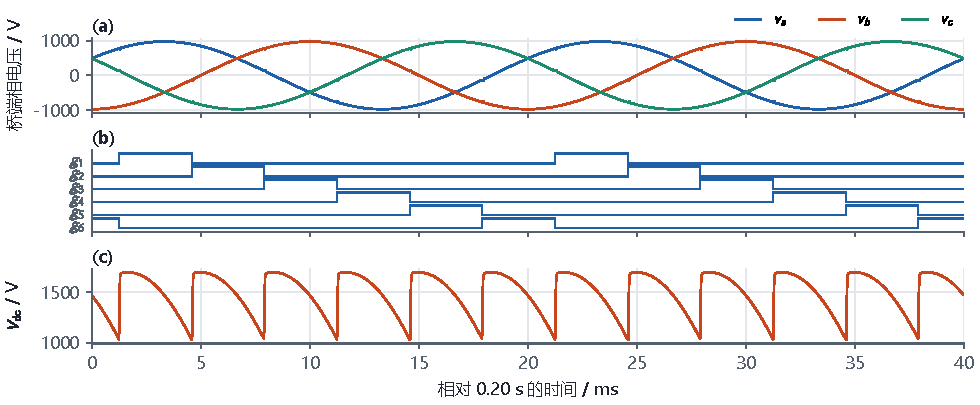
\includegraphics[width=\linewidth]{cs_detail}
\caption{六脉波详细模型 0.20--0.24~s 窗口：(a) 变压器二次侧相电压，(b) 六路门极，(c) 瞬时直流电压}
\label{fig:cs-detail}
\end{figure}

% !TEX root = ../main.tex

\chapter{直流—交流：H 桥电流环}
\label{chap:hb}

\section{主电路}

实验三的对象是电压源型全桥驱动强感性负载、电流闭环的最小完整结构。四只 IGBT 分成两个桥臂，每只反并联一只二极管，C--E 之间并联 10 M$\Omega$ 缓冲电阻；桥臂中点 A、B 之间接 $R=0.2\ \Omega$、$L=20$~mH 的串联负载；直流侧为 2200~V 受控电压源。桥臂状态与输出电压的关系为
\begin{equation}
v\sub{AB}=(s_A-s_B)U\sub{dc},\qquad s_A,s_B\in\{0,1\},
\end{equation}
负载满足
\begin{equation}
L\frac{\dd i}{\dd t}=v\sub{AB}-Ri.
\label{eq:rl}
\end{equation}
式~\eqref{eq:rl} 不含任何控制假设，只要仿真中的 $v\sub{AB}$ 和 $i$ 满足它，功率级和测量链就是自洽的，后文把它作为校核工具。

模型顶层如图~\ref{fig:hb-model} 所示，按给定与使能、电流环与调制、功率级、监视记录四个功能区排列。功率级内部如图~\ref{fig:hb-power}(a) 所示。

\begin{figure}[htbp]
\centering
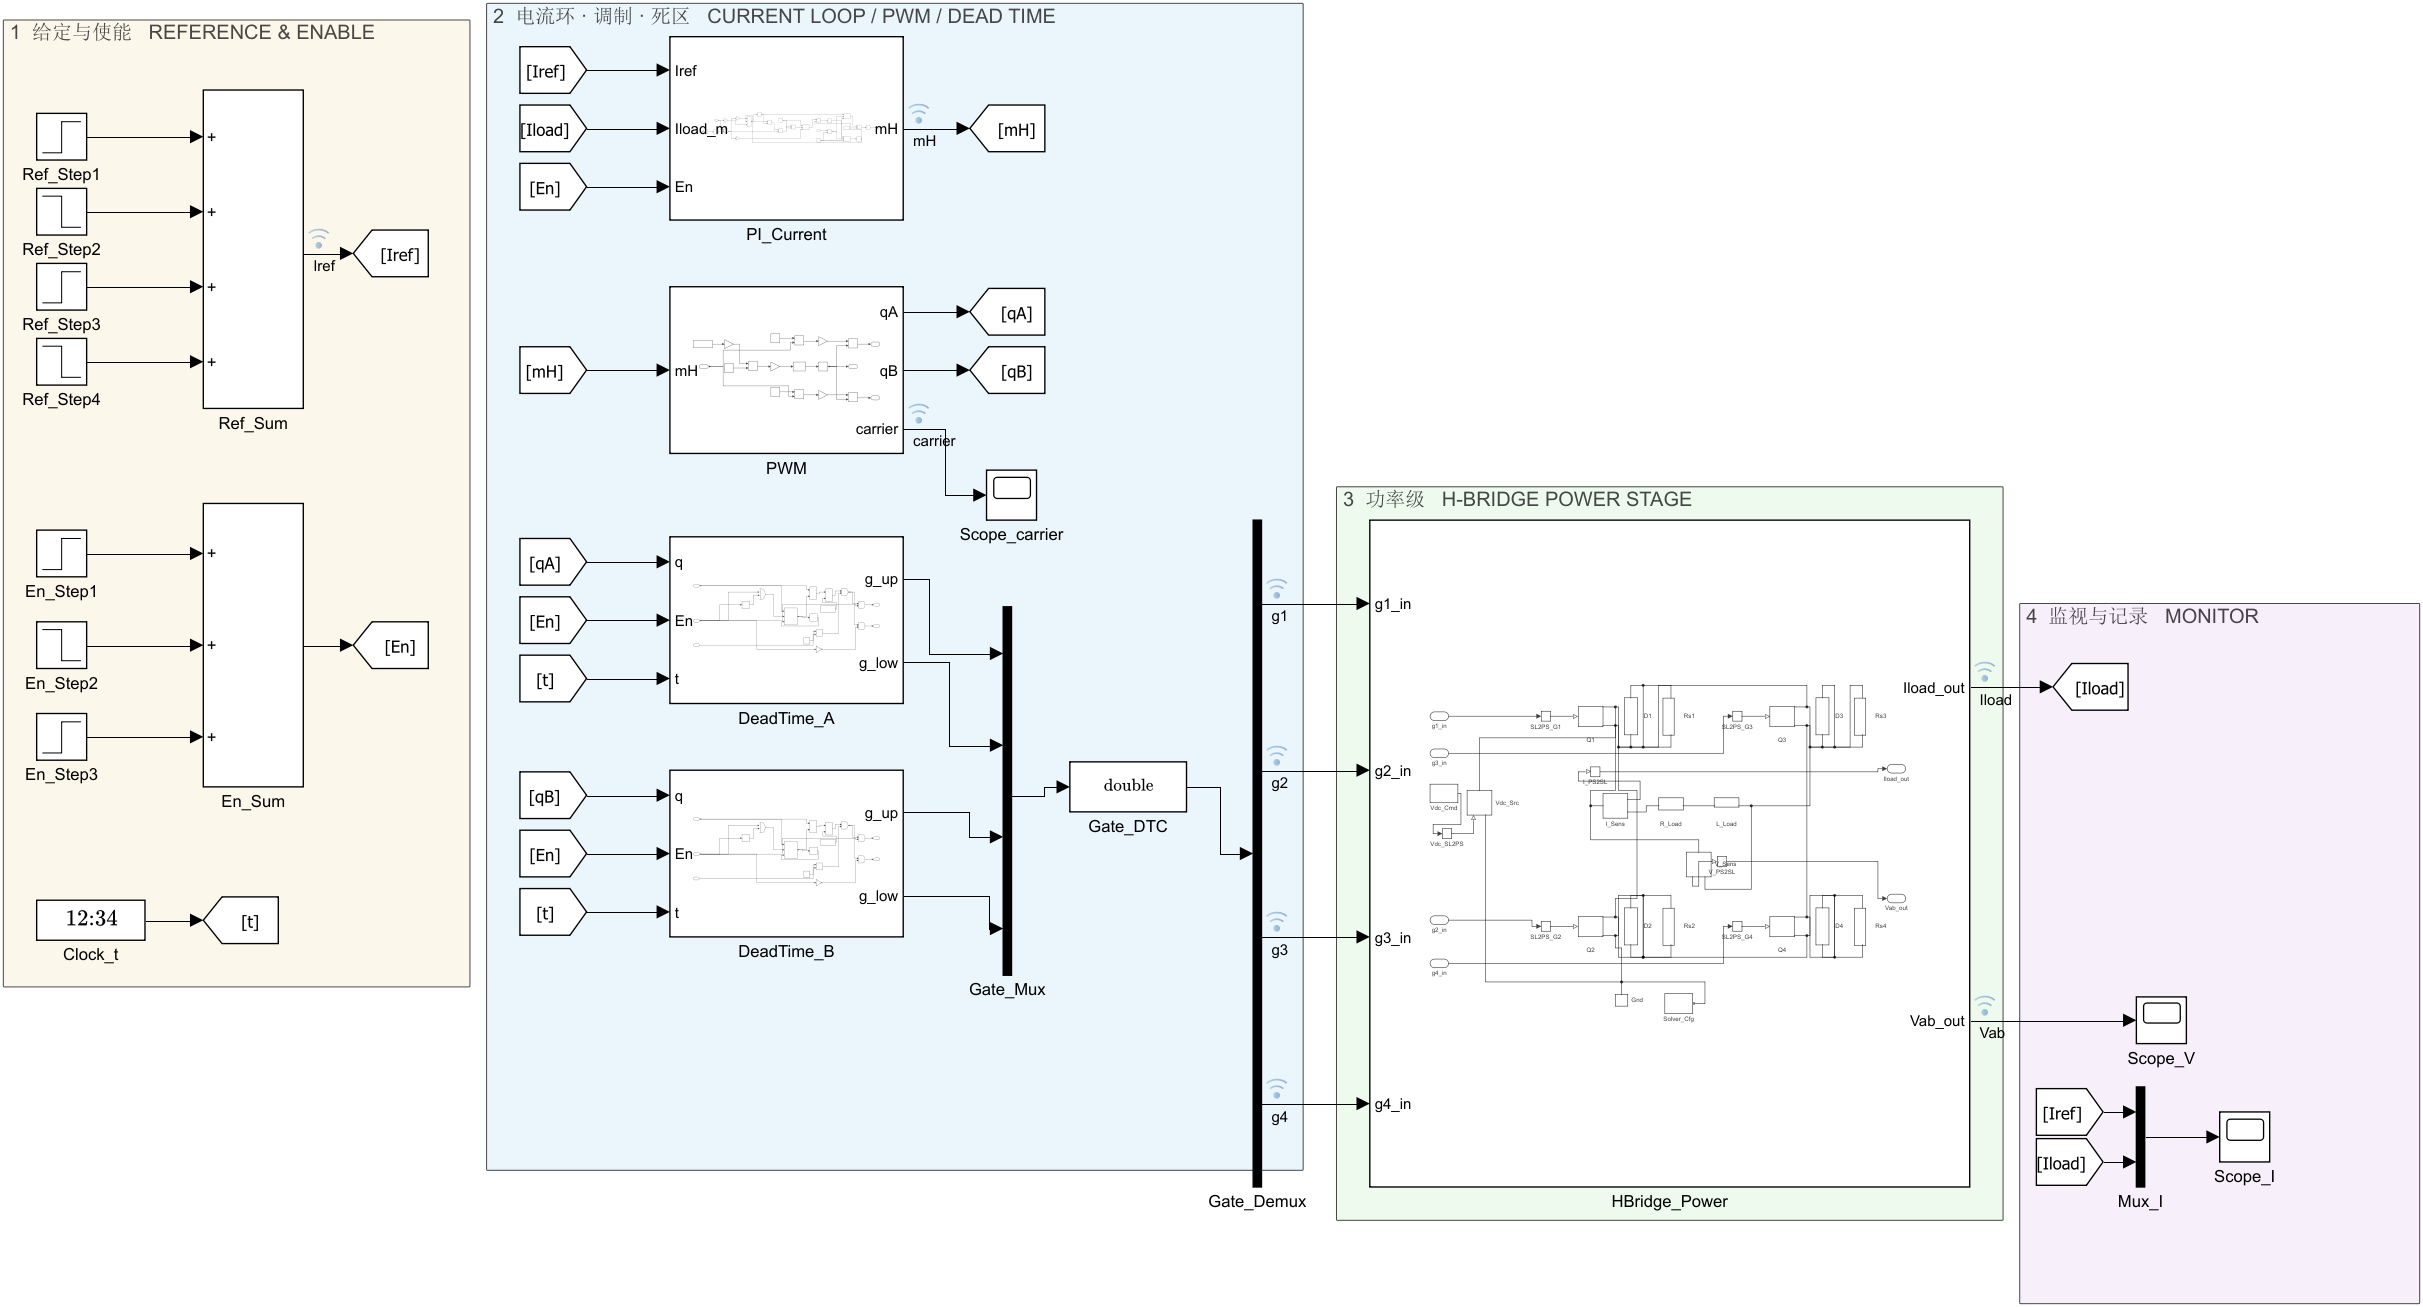
\includegraphics[width=0.74\linewidth]{hb_top.png}
\caption{H 桥模型顶层的四个功能分区（Simulink 原生视图）}
\label{fig:hb-model}
\end{figure}

\sidefig{native/model_hb_power.png}{native/model_deadtime.png}{H 桥模型子系统（Simulink 原生视图）：(a) \texttt{HBridge\_Power} 功率级，(b) 修正后的 \texttt{DeadTime\_A} 死区子系统}{fig:hb-power}

\section{电流环设计}

信号链为传感器、50~$\mu$s 零阶保持、50~$\mu$s 单位延迟和求差。误差分三路进入求和器：比例项 $K_pe$，积分增量 $K_iT_ce$（$T_c=50\ \mu$s），以及电阻压降前馈 $0.2i\sub{ref}$。求和结果限幅 $\pm400$~V，再除以 $U\sub{dc}$ 得到调制比 $m\sub{H}$，并限幅 $\pm0.95$。

参数按零极点对消整定，取 $K_p=\omega_cL$、$K_i=\omega_cR$，则开环传递函数为
\begin{equation}
G\sub{ol}(s)=\Bigl(K_p+\frac{K_i}{s}\Bigr)\frac{1}{Ls+R}=\frac{\omega_c}{s}.
\label{eq:loop}
\end{equation}
穿越频率取 100~Hz，得 $K_p=12.56637$~V/A、$K_i=125.66$~V/(A$\cdot$s)，$K_iT_c=6.2832\times10^{-3}$。抗饱和以限幅前后之差乘以电流误差为判据，结果大于零时把积分增量切为零。使能信号无效时积分状态清零、电压指令切零。图~\ref{fig:hb-pi}(a) 是 0.02~s 阶跃时的内部量：限幅前电压最高为 6268~V，被限到 400~V，积分状态在约 30~ms 的饱和区间内保持为零，退出饱和后才开始积累。

\section{单极性 PWM 与死区}

载波由数字时钟经取模和偏置得到 0--1 三角波，频率 2~kHz、周期 $T_s=500\ \mu$s。两桥臂占空比由同一个 $m\sub{H}$ 映射：
\begin{equation}
d_A=\frac{1+m\sub{H}}{2},\qquad d_B=\frac{1-m\sub{H}}{2},
\end{equation}
各自与同一载波比较。$m\sub{H}>0$ 时输出在 0 和 $+U\sub{dc}$ 之间切换，每个载波周期出现两个脉冲，平均输出电压为
\begin{equation}
\langle v\sub{AB}\rangle=U\sub{dc}\,m\sub{H}.
\label{eq:modlaw}
\end{equation}

死区按“请求变化后延迟 2~$\mu$s 再放行”实现：请求信号与其一拍延迟异或得到变化标志，记住最近一次变化的时刻，当前时间减去该时刻后与 2~$\mu$s 比较，结果再与使能相与（图~\ref{fig:hb-power}(b)）。图~\ref{fig:hb-pwm} 是 $+500$~A 平台 1~ms 的门极、负载电压和电流。负载 $L/R=0.1$~s 远大于载波周期，电流只呈锯齿状纹波，峰峰值 1.0--1.7~A。

原模型直接比较浮点时间差，实测换相间隔会出现 2--3~$\mu$s，只有最小值和中位数恒为 2~$\mu$s。修正版把经过时间先映射回 1~$\mu$s 时钟格点再与 2~$\mu$s 比较，重跑 0.42~s 全部工况后，两个桥臂各 1592 次完整换相的间隔全部为 2~$\mu$s（图~\ref{fig:hb-pi}(b)），门极序列中没有桥臂重叠导通。这一修正随后也用于第 \ref{chap:joint} 章的整机模型。

\begin{figure}[htbp]
\centering
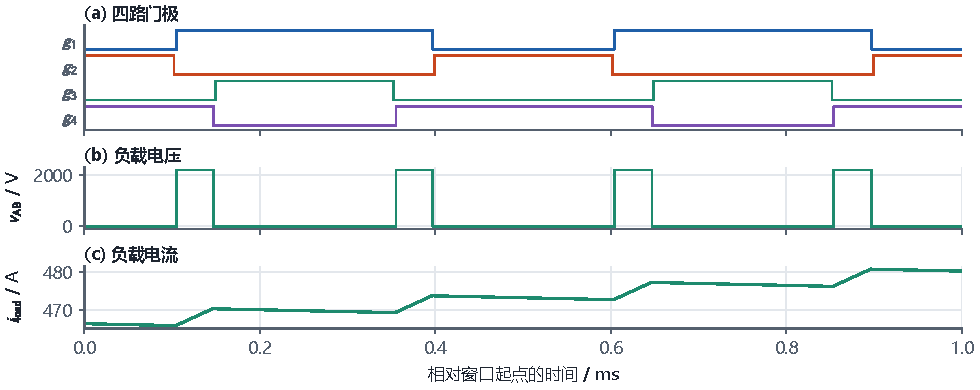
\includegraphics[width=\linewidth]{hb_pwm}
\caption{稳态 $+500$~A 平台：(a) 四路门极，(b) 负载电压，(c) 负载电流纹波}
\label{fig:hb-pwm}
\end{figure}

\twofig{native/hbridge_pi_saturation.pdf}{native/verified_deadtime.pdf}{MATLAB 原生波形：(a) 0.02~s 阶跃时限幅前后的电压指令与积分状态，(b) 修正版两桥臂门极的换相细节}{fig:hb-pi}

\section{五段给定的跟踪结果}

给定由四段阶跃叠加而成：0、$+500$、$-500$、$+300$~A，0.36~s 后回到 0；0.30--0.32~s 之间使能封锁，控制器复位。图~\ref{fig:hb-tracking} 是修正版模型的完整波形，表~\ref{tab:hb-track} 是原模型各段末 20\% 区间的统计。

\begin{figure}[htbp]
\centering
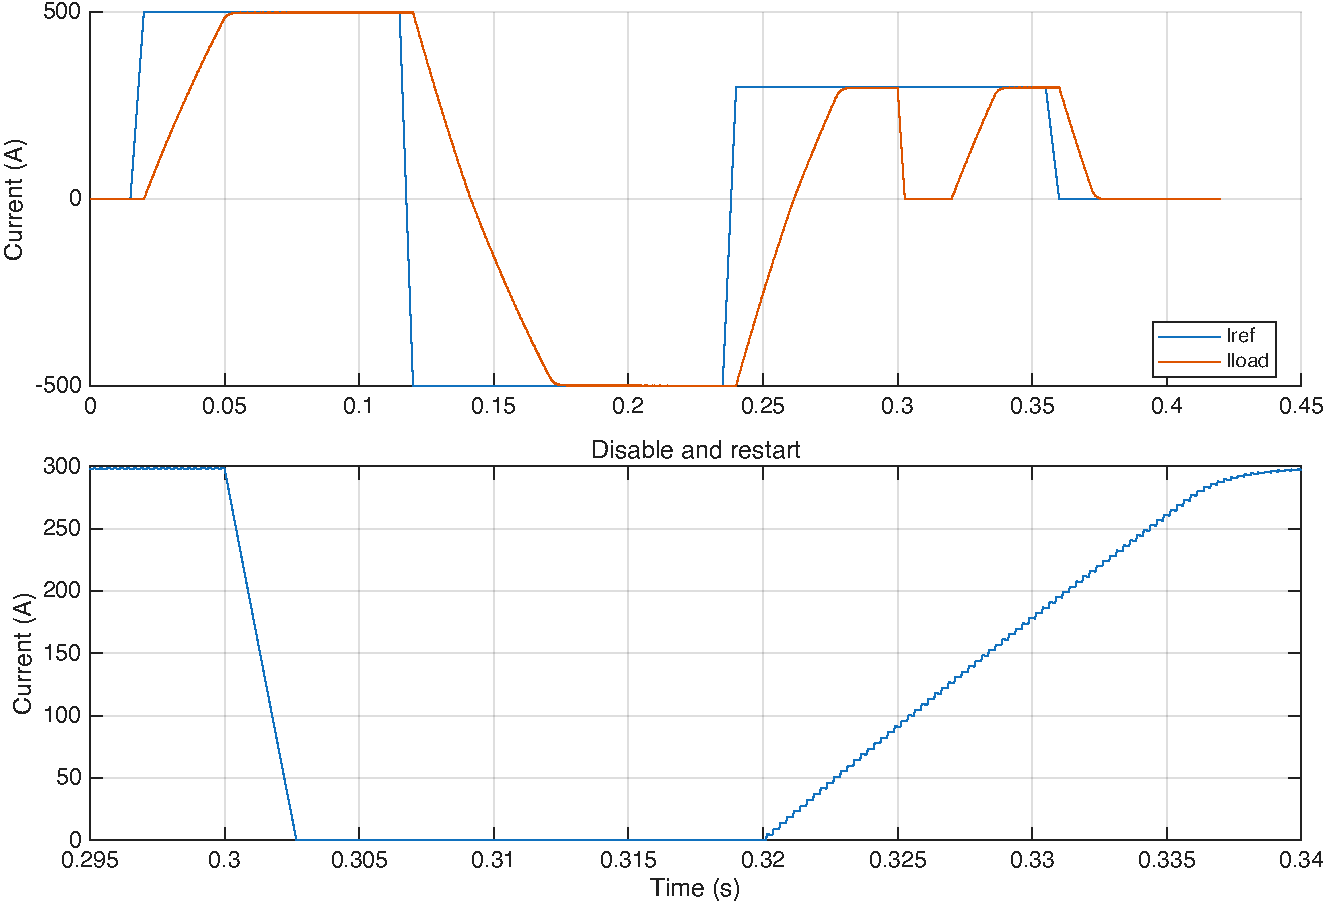
\includegraphics[width=0.68\linewidth]{native/verified_tracking_restart.pdf}
\caption{修正版模型的 MATLAB 原生波形：五段给定跟踪（上）与使能封锁、恢复过程（下）}
\label{fig:hb-tracking}
\end{figure}

\begin{dtable}{htbp}{五段工况的稳态跟踪结果}
\label{tab:hb-track}
\begin{tabularx}{\linewidth}{P{0.36\linewidth}RRRR}
\toprule
\headrow 工况 & $\overline{i\sub{ref}}$ / A & $\overline{i\sub{load}}$ / A & 误差 / A & 纹波 / A \\
\midrule
0~A（0--0.02~s） & 0.03 & 0.000 & 0.03 & 0.00 \\
$+500$~A（0.02--0.12~s） & 500.00 & 499.32 & 0.68 & 1.64 \\
$-500$~A（0.12--0.24~s） & $-499.99$ & $-498.74$ & 1.25 & 1.71 \\
$+300$~A（0.24--0.30~s） & 300.00 & 298.23 & 1.77 & 1.15 \\
$+300$~A（使能 $=0$，0.30--0.32~s） & 300.00 & 0.00 & --- & 0.00 \\
$+300$~A（复位后，0.32--0.36~s） & 300.00 & 298.64 & 1.36 & 1.03 \\
0~A（0.36--0.42~s） & 0.00 & 0.0003 & 0.0003 & 0.0003 \\
\bottomrule
\end{tabularx}
\end{dtable}

方向和幅值都正确，说明电流测量极性、环路符号和 $v\sub{AB}\propto m\sub{H}$ 三者一致。残差的量级也可以解释：死区每个周期造成约 17.6~V 的电压损失，由积分器补偿，而误差通道带有被控对象极点 $s=-R/L$（时间常数 100~ms），残差按 100~ms 衰减。$+500$~A 平台长 100~ms，残差降到 0.68~A；$+300$~A 平台只有 60~ms，结束时还有 1.77~A 且仍在下降。阶跃响应没有超调，$+500$~A 段峰值为 500.12~A，抗饱和起到了作用。

\section{两条独立关系的校核}

把 1~$\mu$s 波形按 500~$\mu$s 分成 840 个窗口，每个窗口对 $v\sub{AB}$、$m\sub{H}$ 和电流取平均。

第一条是调制律。稳态窗口里 $\langle v\sub{AB}\rangle-U\sub{dc}\langle m\sub{H}\rangle$ 的幅值中位数为 18.40~V（正电流段中位数 $-20.0$~V，负电流段 $+18.5$~V），而死区损失为
\begin{equation}
\Delta v=\pm U\sub{dc}\frac{2t_d}{T_s}=\pm2200\times\frac{2\times2\ \mu\mathrm{s}}{500\ \mu\mathrm{s}}=\pm17.60\ \mathrm{V}.
\label{eq:dtvolt}
\end{equation}
偏差符号由电流方向决定，幅值与式~\eqref{eq:dtvolt} 相符（图~\ref{fig:hb-dtvolt}）。按 17.60~V 补偿后残差均方根 7.98~V、最大 14.53~V，不超过 $U\sub{dc}$ 的 0.66\%，其余部分来自器件压降、$m\sub{H}$ 的 50~$\mu$s 离散化和窗口边界效应。

\begin{figure}[htbp]
\centering
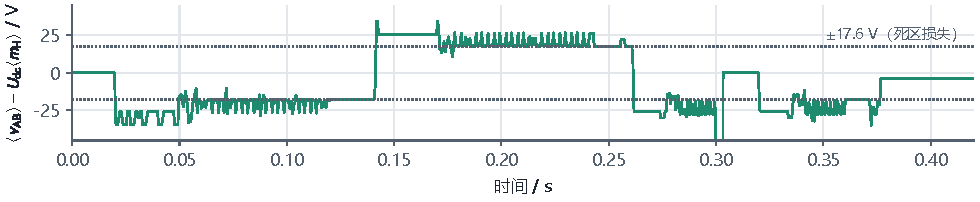
\includegraphics[width=\linewidth]{hb_deadtime_voltage}
\caption{开关周期平均的 $\langle v\sub{AB}\rangle-U\sub{dc}\langle m\sub{H}\rangle$ 在死区损失 $\pm17.6$~V 附近呈台阶状，符号随电流方向改变}
\label{fig:hb-dtvolt}
\end{figure}

第二条是负载回路方程式~\eqref{eq:rl}。对周期平均值做数值微分后，稳态窗口残差的中位数为 0.00~V、均方根为 2.85~V；全部 840 个窗口的最大残差 565~V 出现在阶跃瞬间，属于用窗口平均近似微分的离散化误差。

使能封锁段需要单独解释（图~\ref{fig:hb-tracking} 下）。使能置零后四路门极全为 0，积分状态清零；同臂两管都关断后，感性电流经反并联二极管回馈直流侧，$v\sub{AB}$ 被钳到 $-2204$~V（$-U\sub{dc}$ 减两个二极管压降），电流按 $(-2204-Ri)/L\approx-115$~kA/s 下降，约 2.7~ms 降到零，远快于 $RL$ 无源放电的 100~ms 时间常数。这一段把“控制器复位”和“主电路断开”区分开来：若把封锁理解成断开，就无法解释实测的衰减速度。0.32~s 使能恢复后，电流在 40~ms 内重新跟到 298.64~A。

% !TEX root = ../main.tex

\chapter{负载侧：可变等离子体负载}
\label{chap:plasma}

\section{互感耦合回路}

实验四把 H 桥的负载由线性支路换成“原边线圈 + 副边等离子体回路”的耦合结构（图~\ref{fig:pl-model}）。原边从桥臂 A 出发，串入 $i\sub{cs}$ 测量和 20 $\mu\Omega$ 的电阻 $R\sub{cs}$，接到互感原边绕组后回到桥臂 B。副边经 $i\sub{p}$ 测量、可变电感 $L\sub{p}(t)$、可变电阻 $R\sub{p}(t)$ 构成回路。两支 100~k$\Omega$ 电阻分别并在 $L\sub{p}$ 和 $R\sub{p}$ 两端，只起数值作用。

\begin{figure}[htbp]
\centering
\begin{circuitikz}[font=\footnotesize, line width=0.55pt, >={Latex[length=1.5mm]}]
\ctikzset{bipoles/length=0.95cm, resistors/scale=0.75, inductors/scale=0.75, diodes/scale=0.75, sources/scale=0.8}
\newcommand{\qd}[4]{% x, y of collector, name, diode side
  \node[nigbt, anchor=C, scale=0.72] (#3) at (#1,#2) {};
  \draw (#3.E) -- ++(#4,0) coordinate (#3e) to[D*] ($(#3.C)+(#4,0)$) -- (#3.C);
}
\draw (-1.3,0) to[V, l=$U\sub{dc}$, invert] (-1.3,5) ;
\draw[line width=0.8pt] (-1.3,5) -- (9.4,5);
\draw[line width=0.8pt] (-1.3,0) -- (9.4,0);
\qd{0.6}{4.55}{Q1}{0.72}
\qd{0.6}{1.8}{Q2}{0.72}
\qd{9.4}{4.55}{Q3}{0.72}
\qd{9.4}{1.8}{Q4}{0.72}
\draw (0.6,5) -- (Q1.C);
\draw (Q1.E) -- (Q2.C) node[midway,circ] (A) {};
\draw (Q2.E) -- (0.6,0);
\draw (9.4,5) -- (Q3.C);
\draw (Q3.E) -- (Q4.C) node[midway,circ] (B) {};
\draw (Q4.E) -- (9.4,0);
\node[above left=0pt and 0pt of A, font=\footnotesize] {A};
\node[above right=0pt and 0pt of B, font=\footnotesize] {B};
\node[font=\scriptsize, text=inkmuted] at ($(Q1.G)+(-0.2,0)$) {$Q_1$};
\node[font=\scriptsize, text=inkmuted] at ($(Q2.G)+(-0.2,0)$) {$Q_2$};
\node[font=\scriptsize, text=inkmuted] at ($(Q3.G)+(-0.2,0)$) {$Q_3$};
\node[font=\scriptsize, text=inkmuted] at ($(Q4.G)+(-0.2,0)$) {$Q_4$};
\draw (A) to[short, i=$i\sub{cs}$] (1.95,0 |- A) to[R, l=$R\sub{cs}$] (3.1,0 |- A) -- (3.45,0 |- A) -- (3.45,3.55);
\coordinate (p1) at (3.45,3.55); \coordinate (p2) at (3.45,1.35);
\draw (p1) to[L, l_=$L_1$] (p2);
\draw (p2) -- (3.45,0.65) -- (8.75,0.65) -- (8.75,0 |- B) -- (B);
\coordinate (s1) at (4.35,3.55); \coordinate (s2) at (4.35,1.35);
\draw (s1) to[L, l=$L_2$] (s2);
\draw[<->, line width=0.45pt, color=inkmuted] (3.62,3.75) to[bend left=25] node[above, font=\scriptsize] {$k=0.99999$} (4.18,3.75);
\draw (s1) to[short, i=$i\sub{p}$] (5.25,3.55) to[vL, l=$L\sub{p}(t)$] (7.3,3.55) -- (7.75,3.55) to[vR, l=$R\sub{p}(t)$] (7.75,1.35) -- (s2);
\end{circuitikz}
\caption{H 桥与互感耦合可变负载的主电路（数值并联电阻和缓冲电阻未画出）}
\label{fig:pl-model}
\end{figure}

两绕组自感都是 1~H、耦合系数 $k=0.99999$，可以近似为理想变压器。励磁电流和磁链为
\begin{equation}
i\sub{m}=i\sub{cs}-i\sub{p},\qquad \psi=L_1i\sub{m}.
\label{eq:flux}
\end{equation}
忽略 $R\sub{cs}$ 上的压降，原边和副边分别满足
\begin{equation}
u\sub{AB}=\frac{\dd\psi}{\dd t},\qquad
\frac{\dd\psi}{\dd t}=R\sub{p}(t)\,i\sub{p}+L\sub{p}(t)\frac{\dd i\sub{p}}{\dd t}.
\label{eq:pl-loop}
\end{equation}
等离子体电流由磁链变化率驱动，稳态时 $i\sub{p}\approx u\sub{AB}/R\sub{p}$。$R\sub{p}$ 只有 0.01~$\Omega$，所以百伏级的桥臂电压就能维持上万安的电流；12.3~s 之后 $R\sub{p}$ 升到 100~$\Omega$，副边回路事实上被断开，这时必须由原边主动把磁链拉回零，即“退磁”。

$R\sub{p}$ 和 $L\sub{p}$ 由同一时钟驱动的两张一维查表给出，线性插值、截断外插（图~\ref{fig:pl-schedule}(a)）。两绕组的短路电感 $L_\sigma=2L_1(1-k)\approx20\ \mu$H，与 $L\sub{p}$ 串联后，副边回路的等效串联电感在启动段约 170~$\mu$H，平台段约 120~$\mu$H。$L\sub{p}$ 的变化安排在 0.6--1.6~s 的启动段，与电流上升同时进行，这一段 $L\sub{p}\,\dd i\sub{p}/\dd t$ 不超过 1.5~V，对平台段没有影响。Simulink 中的功率级实现如图~\ref{fig:pl-schedule}(b) 所示。

\sidefig{native/plasma_load_schedule.pdf}{native/model_plasma_power.png}{(a) 副边可变参数的时序（MATLAB 原生波形），(b) \texttt{Power\_Stage} 子系统（Simulink 原生视图）}{fig:pl-schedule}

\section{控制策略}

反馈量由负载电流换成等离子体电流，控制结构仍是“采样—比例积分—前馈—限幅—抗饱和”（图~\ref{fig:pl-pi}），但参数必须重新整定。被控对象的直流增益由 $1/R=5$~A/V 变为 $1/R\sub{p}\approx100$~A/V，时间常数由 100~ms 变为 $L_{\sigma,\mathrm{eq}}/R\sub{p}\approx12$--$17$~ms。沿用实验三的 $K_p=12.57$~V/A 时，穿越频率会超过 10~kHz，高于 PWM 载波，闭环无法稳定。

仍按零极点对消、$\omega_c=2\pi\times100$ rad/s 整定，$K_p=\omega_cL_{\sigma,\mathrm{eq}}\approx0.107$~V/A、$K_i=\omega_cR\sub{p}\approx6.28$~V/(A$\cdot$s)，模型取整为 $K_p=0.1$、$K_i=6.25$。前馈项取 $R\sub{p}(t)i\sub{ref}$，平台段约 100~V，正好是回路电压，积分器只需补偿纹波和器件压降。电压指令限幅 $\pm400$~V，调制比限幅 $\pm0.95$，抗饱和判据与实验三相同。

\begin{figure}[htbp]
\centering
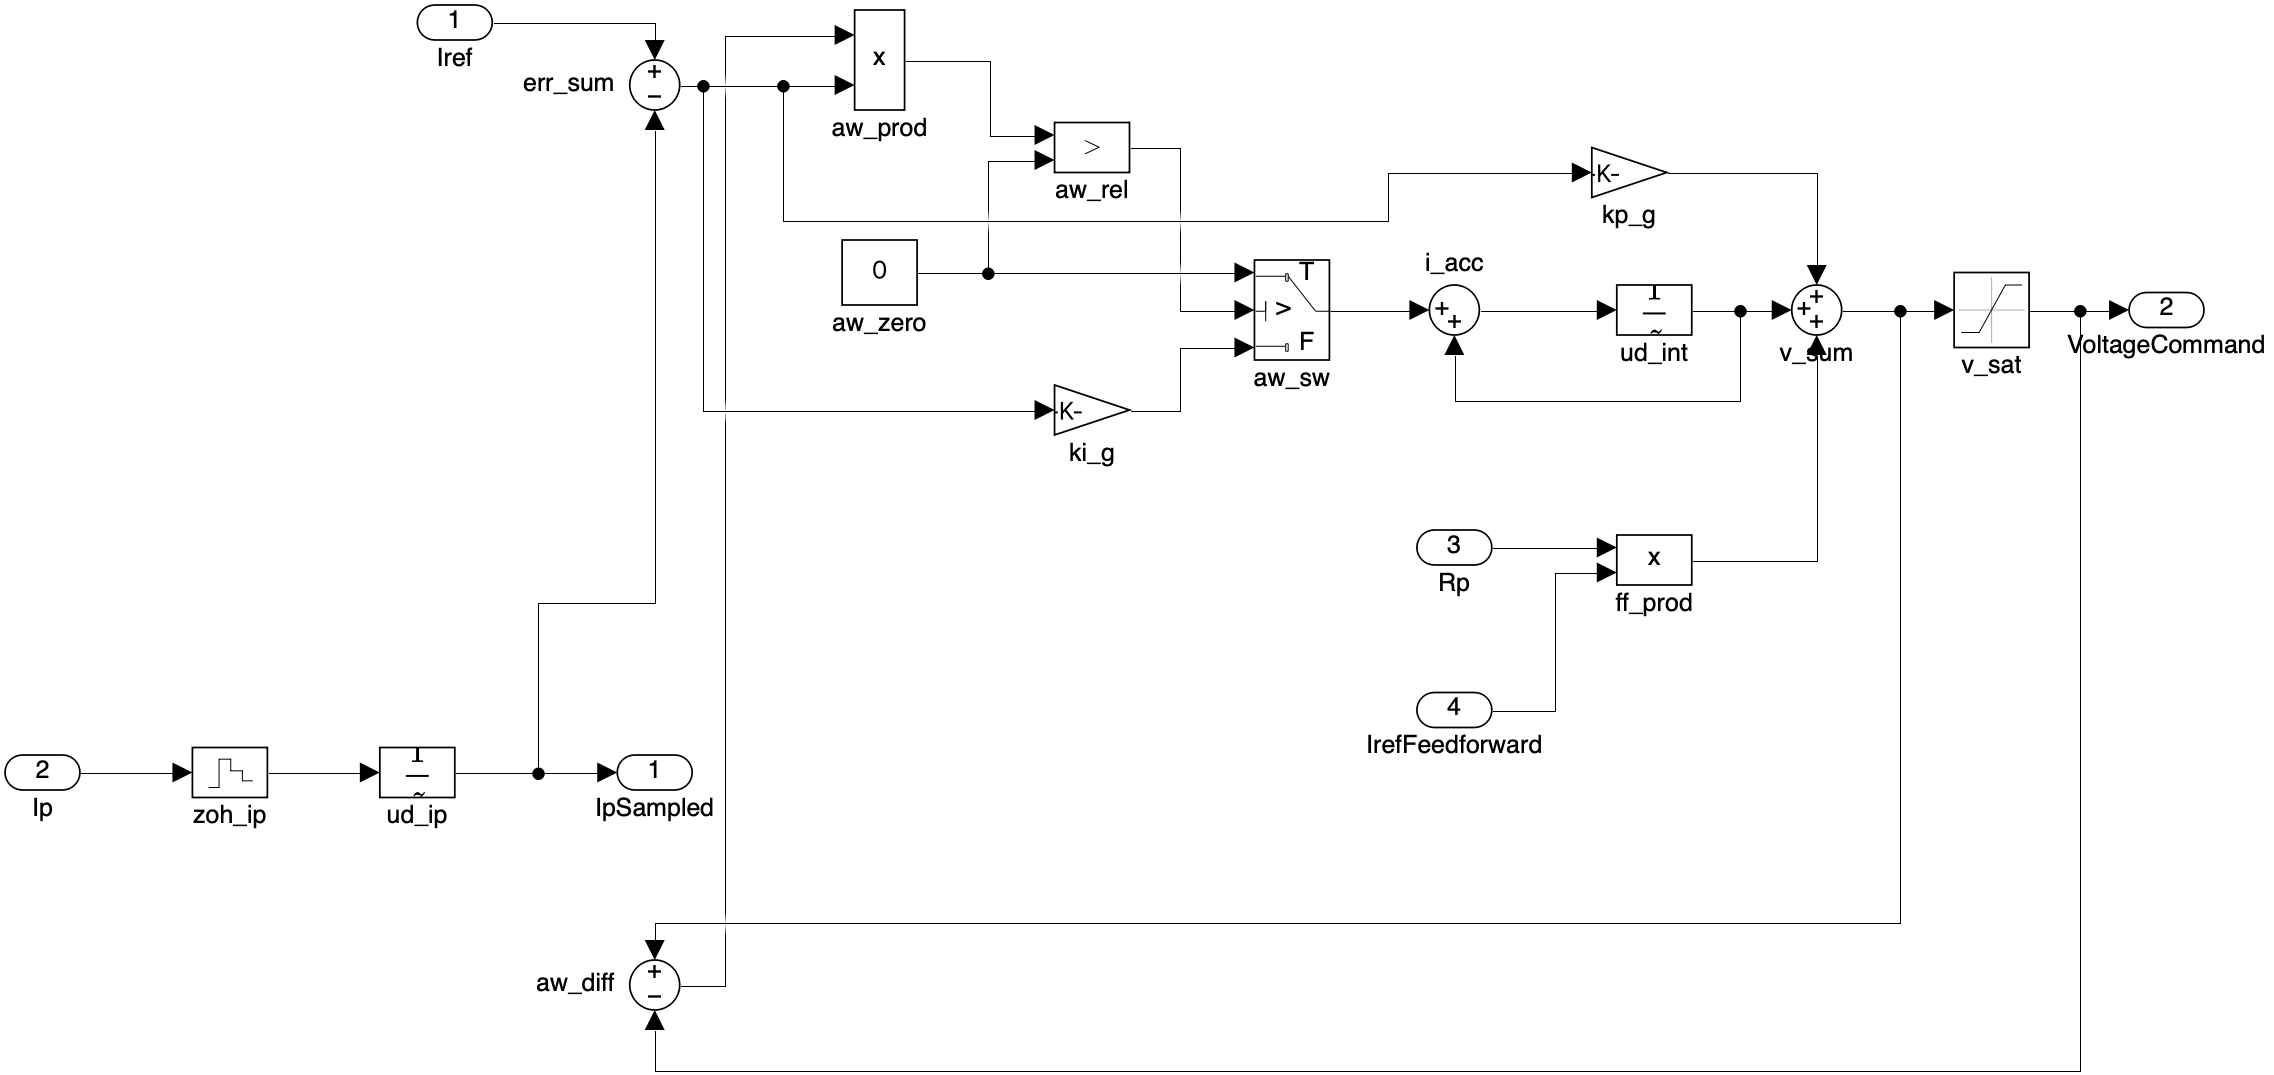
\includegraphics[width=0.56\linewidth]{native/model_current_pi.png}
\caption{\texttt{Current\_PI} 子系统（Simulink 原生视图）：比例积分、抗饱和判据与 $R\sub{p}i\sub{ref}$ 前馈}
\label{fig:pl-pi}
\end{figure}

12.3~s 起切换为退磁控制，被控量改成励磁电流：
\begin{equation}
\hat\psi=L_1(i\sub{cs}-i\sub{p}),\qquad u^{\mathrm{demag}}\sub{AB}=-k_\psi\hat\psi,\quad k_\psi=2\ \mathrm{V/Wb}.
\label{eq:demag}
\end{equation}
纯比例律使磁链按 $1/k_\psi=0.5$~s 的时间常数衰减，输出电压同样限幅 $\pm400$~V。模式切换由受退磁标志控制的 Switch 完成，$i\sub{cs}$ 和 $i\sub{p}$ 先经 50~$\mu$s 采样再进入退磁控制，以避免代数环。

\section{基线模型的运行结果}

实验四的基线模型运行在 2200~V 理想母线上，步长 10~$\mu$s，载波 4~kHz（指导书未重新指定载波频率，基线沿用原设置）。结果见图~\ref{fig:pl-wave} 和表~\ref{tab:pl-plateau}，表中同时列出第 \ref{chap:joint} 章整机模型的同口径结果。

\twofig{native/plasma_startup.pdf}{native/plasma_full_pulse.pdf}{基线模型的 MATLAB 原生波形：(a) 启动段跟踪，(b) 30~s 全过程的电流与功率}{fig:pl-wave}

\begin{dtable}{htbp}{平台段（6--11~s）统计：基线模型与整机模型}
\label{tab:pl-plateau}
\begin{tabularx}{\linewidth}{LRRL}
\toprule
\headrow 物理量 & 基线模型 & 整机模型 & 说明 \\
\midrule
直流母线 & 2200~V & 2199.98~V & 理想源 / 实际母线 \\
载波与步长 & 4~kHz，10~$\mu$s & 2~kHz，1~$\mu$s & 整机含 2~$\mu$s 死区 \\
等离子体电流 $\bar i\sub{p}$ & 10\,006.91~A & 9\,999.28~A & 给定 10~kA \\
线圈电流 $\bar i\sub{cs}$ & 10\,756.87~A & 10\,749.17~A & 含励磁分量约 750~A \\
线圈侧功率 & 1.0879~MW & 1.0781~MW & 桥臂输出 \\
等离子体功率 & 1.0014~MW & 约 1.000~MW & $R\sub{p}i\sub{p}^2$ \\
电流纹波峰峰值 & 304.03~A & 226.55~A & 1.8--1.85~s 窗口 \\
\bottomrule
\end{tabularx}
\end{dtable}

\textbf{启动段。}0.6~s 之前使能为 0、门极封锁；0.6~s 起给定按 10~kA/s 上升，$i\sub{p}$ 几乎无滞后地跟随，1.6~s 到达 10~kA。$u\sub{AB}$ 只需在 0--100~V 之间变化，离限幅很远，整段都是小信号工作。

\textbf{平台段。}$i\sub{cs}$ 由 1.6~s 的约 10.05~kA 爬升到 11.6~s 的约 11.05~kA，增量约 1~kA，正好是励磁电流的增长：磁链以 $R\sub{p}i\sub{p}\approx100$~V 的速率被消耗，$i\sub{m}=\psi/L_1$ 随时间线性增长。线圈侧与等离子体侧的功率差主要是励磁储能的增长率 $i\sub{m}\dd\psi/\dd t\approx750\ \mathrm{A}\times100\ \mathrm{V}=75$~kW，加上 $R\sub{cs}i\sub{cs}^2\approx2.3$~kW 的电阻损耗，合计 77.3~kW。1~$\mu$s 的整机模型实测差值约 78~kW，与之相符；10~$\mu$s 基线为 86.5~kW，偏大的部分与较粗步长下的开关量化有关。

\textbf{降流与退磁。}11.6~s 起给定以 20~kA/s 下降，0.5~s 内跟到零。12.1~s 起 $R\sub{p}$ 在 0.2~s 内升到 100~$\Omega$，12.3~s 切入退磁。开始时 $\hat\psi$ 较大，退磁律输出顶到 $-400$~V，磁链以约 400~Wb/s 的恒定速率下降，$i\sub{cs}$ 由约 1.08~kA 近似线性回落（图~\ref{fig:pl-flux}(a)）。线圈侧在 12.3--30~s 向直流侧净回馈 0.565~MJ。

基线的退磁尾段值得注意：15.5--24~s 内 $i\sub{cs}$ 由 44~A 匀速降到约 9~A，斜率恰为 4~A/s，桥臂输出恒为 $-4.0$~V，对应两只器件的压降。说明此时指令很小，脉宽已低于 10~$\mu$s 步长可分辨的范围，磁链主要靠器件压降衰减。1~$\mu$s 的整机模型没有这一现象，电流按指数收尾，16~s 时已降到 3.9~A。

\twofig{native/plasma_demagnetization.pdf}{native/plasma_flux_crosscheck.pdf}{基线模型的 MATLAB 原生波形：(a) 降流与退磁段的电流和线圈侧功率，(b) 磁链两条路径及其残差}{fig:pl-flux}

\section{数值校核}

磁链的两条路径是这个模型最有价值的校核（图~\ref{fig:pl-flux}(b)）。一条用电流计算，$\psi_i=L_1(i\sub{cs}-k\,i\sub{p})$；另一条用原生 10~$\mu$s 实测电压积分，$\psi_u=\int(v\sub{AB}-R\sub{cs}i\sub{cs})\,\dd t$。全程最大残差约 0.011~Wb，而平台段磁链变化量为 991~Wb。这一比较说明互感参数填写正确、原副边电流方向一致，$L\sub{p}$ 和 $R\sub{p}$ 确实串联在副边回路中，没有被 100~k$\Omega$ 并联支路旁路。

\textbf{电流纹波。}单极性调制下每半个载波周期出现一个电压脉冲，平台段的纹波可以估计为
\begin{equation}
\Delta i\sub{p}\approx\bar u\Bigl(1-\frac{\bar u}{U\sub{dc}}\Bigr)\frac{T_s}{2L_{\sigma,\mathrm{eq}}},
\label{eq:pl-ripple}
\end{equation}
取 $\bar u=100$~V、$L_{\sigma,\mathrm{eq}}=120\ \mu$H，2~kHz 时约为 200~A（2\%），4~kHz 时约为 100~A。表~\ref{tab:pwm} 是同一负载在不同载波和步长下的实测结果，图~\ref{fig:pwm} 是对应的波形。

\begin{dtable}{htbp}{PWM 设置与求解步长对电流纹波的影响（均为 30~s 运行）}
\label{tab:pwm}
\begin{tabularx}{\linewidth}{P{0.46\linewidth}RRR}
\toprule
\headrow 工况 & 平台段 $\bar i\sub{p}$ / A & 纹波峰峰值 / A & 式~\eqref{eq:pl-ripple} 估计 / A \\
\midrule
基线：4~kHz，10~$\mu$s，无死区 & 10\,006.91 & 304.03 & 100 \\
2~kHz，10~$\mu$s，无死区 & 10\,004.37 & 559.55 & 200 \\
2~kHz，1~$\mu$s，原死区实现（2--3~$\mu$s） & 9\,999.19 & 245.47 & 200 \\
整机：2~kHz，1~$\mu$s，修正死区（2~$\mu$s） & 9\,999.28 & 226.55 & 200 \\
\bottomrule
\end{tabularx}
\end{dtable}

平台段脉宽只有约 6--12~$\mu$s，10~$\mu$s 步长会把脉宽量化放大，所以 10~$\mu$s 的纹波明显偏离估计，也不能据此比较载波频率的影响。步长减到 1~$\mu$s 后，实测值接近估计，余下的差异与死区展宽脉冲有关。因此，本报告把 1~$\mu$s 工况的约 2.3\% 作为电流纹波的代表值。

\begin{figure}[htbp]
\centering
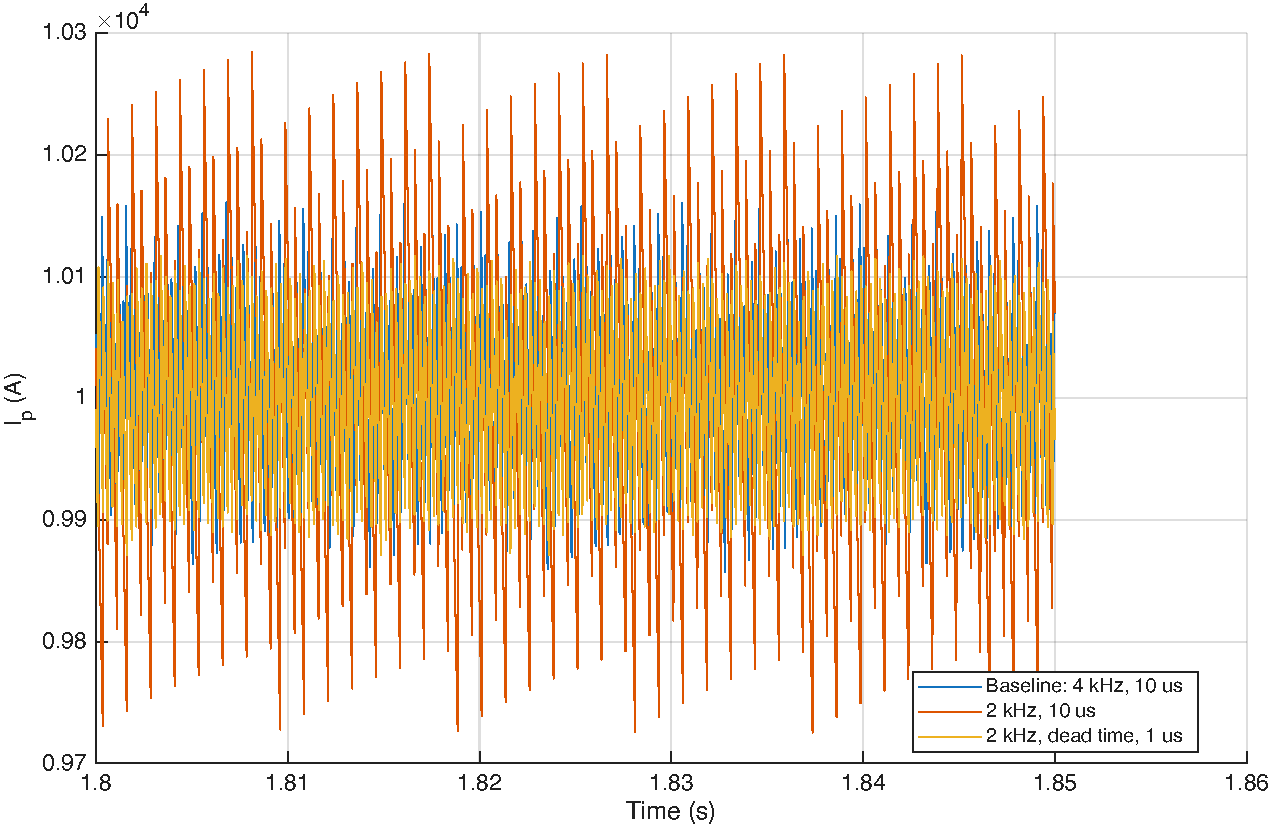
\includegraphics[width=0.5\linewidth]{native/pwm_current_ripple.pdf}
\caption{三种 PWM 设置下 1.8--1.85~s 的电流纹波（MATLAB 原生波形）}
\label{fig:pwm}
\end{figure}

% !TEX root = ../main.tex

\chapter{全链路联合仿真}
\label{chap:joint}

\section{系统整合}

前述模型之间都隔着一个理想电源，后级负载无法影响前级。整机模型去掉 2200~V 理想电压源，把各环节放进同一个 Simscape 电气网络：10~kV 下垂调压电源经源阻抗和 10/1~kV 变压器接到双向平均值 AC/DC，直流母线接开关级 H 桥，H 桥驱动互感耦合的可变负载。退磁能量可以沿同一网络返回交流侧。

模型顶层如图~\ref{fig:int-model}(a) 所示，分为交直流供电、功率级、控制器、负载时序、时钟和观测六部分；供电子系统如图~\ref{fig:int-model}(b) 所示。表~\ref{tab:joint-map} 列出各环节的来源及整合时的处理。

\sidefig{native/model_int_system.png}{native/model_int_acdc.png}{整机模型（Simulink 原生视图）：(a) 顶层 \texttt{tokamak\_integrated}，(b) \texttt{ACDC\_Supply} 子系统}{fig:int-model}

\begin{dtable}{htbp}{已有模型到整机模型的映射}
\label{tab:joint-map}
\begin{tabularx}{\linewidth}{P{0.13\linewidth}P{0.36\linewidth}L}
\toprule
\headrow 来源 & 保留内容 & 整合处理 \\
\midrule
实验二 & 10~kV 电源、电网阻抗、无功下垂与电压 PI & 测试负载换成 10/1~kV 变压器和 AC/DC \\
实验三 & 四管 H 桥、单极性 PWM、2~kHz 载波、2~$\mu$s 死区 & 采用修正后的死区子系统，以 1~$\mu$s 求解 \\
实验四 & 电流 PI、互感回路、变参数时序、退磁控制 & 移除理想 2200~V 电源，接入实际母线 \\
新增 & 双向平均值 AC/DC，20~mF 直流缓冲电容 & 属于本项目的接口建模假设 \\
\bottomrule
\end{tabularx}
\end{dtable}

\section{双向平均值接口}

接口采用理想电网同步参考（频率 50~Hz，相位与电源相同），不模拟锁相环、整流器开关、滤波器和器件损耗。令 $\theta=2\pi\times50t$，变比 $r=2200/1000=2.2$，开关函数向量为
\begin{equation}
\boldsymbol m=r\sqrt{\tfrac23}\begin{bmatrix}\sin\theta&\sin(\theta-\tfrac{2\pi}{3})&\sin(\theta+\tfrac{2\pi}{3})\end{bmatrix}^{\mathrm T}.
\end{equation}
端口关系为
\begin{equation}
V\sub{dc}=\boldsymbol m^{\mathrm T}\boldsymbol v\sub{abc},\qquad \boldsymbol i\sub{ac}=-\boldsymbol m\,i\sub{dc},
\label{eq:acdc}
\end{equation}
其中 $i\sub{dc}$ 以流入变换器直流正端为正，于是每一时刻都有 $\boldsymbol v\sub{abc}^{\mathrm T}\boldsymbol i\sub{ac}+V\sub{dc}i\sub{dc}=0$：功率可以双向传递，接口自身不储能。对与参考同相的平衡正弦电压，$V\sub{dc}=rV\sub{LL,rms}$。

这是理想变换级的聚合关系，变比并不代表某个已设计好的两电平整流器能够实现该增益。20~mF 缓冲电容预充至 2200~V（初始储能 48.4~kJ）。2200~V 是接口额定点，实际母线电压随交流侧变化；电流环仍按名义 2200~V 换算调制比，没有增加直流母线外环。

全局求解器为固定步长 ode3，步长 1~$\mu$s，Simscape 局部后向欧拉每步 3 次非线性迭代；30~s 工况实际耗时约 16~min。死区判断先映射回 1~$\mu$s 时钟格点（第 \ref{chap:hb} 章）。综合信号每 10~$\mu$s 记录一次，能量在模型内部按 1~$\mu$s 积分，报告中的能量都取自这些积分通道。

\section{全程运行结果}

整机从零时刻连续运行到 30~s，覆盖升流、平台、降流与退磁（图~\ref{fig:int-wave}），平台段统计见表~\ref{tab:int-platform}。$i\sub{p}$ 均值 9999.28~A，跟踪给定 10~kA；全程结束时线圈电流约 $-4.2\times10^{-8}$~A，磁链回到零。母线全程在 2187.0--2219.2~V 之间，只偏离额定点约 $\pm1\%$，峰值出现在 12.3~s 切入退磁的瞬间。

\twofig{native/int_currents_dc.pdf}{native/int_power_energy.pdf}{整机 30~s 运行的 MATLAB 原生波形：(a) 等离子体电流、线圈电流和母线电压，(b) 各级功率与净能量}{fig:int-wave}

\begin{dtable}{htbp}{整机运行的平台段统计（6--11~s）}
\label{tab:int-platform}
\begin{tabularx}{\linewidth}{P{0.26\linewidth}RP{0.26\linewidth}R}
\toprule
\headrow 指标 & 数值 & 指标 & 数值 \\
\midrule
母线电压平均值 & 2199.98~V & 交流侧有功 & 1.1259~MW \\
母线电压最小 / 最大 & 2199.08 / 2200.83~V & 交流侧无功 & $-0.012$~Mvar \\
等离子体平均电流 & 9999.28~A & 线圈侧功率 & 1.0781~MW \\
原边平均电流 & 10\,749.17~A & 交流母线电压 & 1.00005~pu \\
直流侧电流平均值 & 512.2~A & 内部电势 & 1.0022~pu \\
\bottomrule
\end{tabularx}
\end{dtable}

交流母线电压 1.00005~pu，与由 $Q=-0.012$~Mvar 计算的下垂目标 1.00006~pu 一致；无功接近零，因此下垂几乎不动作，内部电势只需抬高 0.22\% 以补偿有功电流的阻抗压降（图~\ref{fig:int-grid}(a)）。接口是平均值模型且假设同步，这个结果不能理解为全工况单位功率因数，负载造成端口电压相移时无功并不严格为零。

\section{能量闭合与退磁回馈}

理想接口使交流侧与直流侧的累计能量完全相等，功率残差不超过 $10^{-9}$ W，缓冲电容净储能变化可以忽略。全程净能量：交流侧与直流侧 11.1059~MJ，线圈侧 10.5964~MJ，差值 0.5095~MJ 是 H 桥器件损耗。

\twofig{native/int_grid_response.pdf}{native/int_demag_return.pdf}{MATLAB 原生波形：(a) 交流侧电压、功率与负载时序，(b) 退磁段的电流、功率和自 12.3~s 起的净能量}{fig:int-grid}

退磁段的能量逐级可以对上（图~\ref{fig:int-grid}(b)）。互感磁场储能峰值 $\tfrac12L_1i\sub{m}^2=0.588$~MJ；12.3--30~s 线圈向 H 桥净回馈 0.565~MJ，向交流侧净回馈 0.559~MJ，逐级减少的部分对应 $R\sub{cs}$ 和器件损耗。

\section{门极、纹波与数值检查}

启动（1.98--2~s）和末段（29.98--30~s）两个 1~$\mu$s 门极窗口都测得 2~$\mu$s 死区，桥臂重叠导通的记录数为 0（图~\ref{fig:int-gate}(b)）。平台段电流纹波峰峰值 226.55~A，母线上对应约 $\pm3$~V 的开关纹波（图~\ref{fig:int-gate}(a)）。

启动工况把每步非线性迭代由 3 次增加到 6 次，两路电流的最大绝对差约 $1.45\times10^{-8}$~A。这只是该工况的数值敏感性检查，并不构成全工况的收敛证明。四个基线模型在布局整理前后做了逐点比较，保存的信号和 Simscape 日志完全一致，这一结论只针对基线的布局整理，不适用于改变了功能的修正版和整机模型。

\twofig{native/int_current_dc_ripple.pdf}{native/int_deadtime_zoom.pdf}{MATLAB 原生波形：(a) 1.8--1.82~s 的等离子体电流和母线电压纹波，(b) 两桥臂换相的 2~$\mu$s 死区}{fig:int-gate}

\section{晶闸管整流接口的对照}

项目同时保留了另一套联合模型（分支 \texttt{task05-system-integration}），接口采用真实的六晶闸管全控桥：10/1.2~kV 变压器、5~mH 平波电抗器、0.2~F 母线电容，目标电压 1500~V，功率级步长 2~$\mu$s。桥只能单向供能，退磁能量无法回到电网，因此增设滞环制动支路：母线达到 1650~V 时投入 5~$\Omega$ 电阻，降到 1600~V 时退出。

这一接口带来了平均值模型中没有的问题。空电容直接充电时母线峰值约 2.58~kV，为此把电压参考改为 0--0.5~s 线性上升，并引入 0.01 $^\circ$/A 的电流阻尼（图~\ref{fig:thy}(a)）。退磁回馈约 0.56~MJ，电容从 1500~V 升到 1650~V 只能吸收 47.25~kJ，其余由制动电阻消耗（图~\ref{fig:thy}(b)）。降流开始后 H 桥不再取用功率，电压环把触发角推到 $85^\circ$ 上限，整流器基本停止输出（图~\ref{fig:thy}(c)）。平台段平均触发角 19.42$^\circ$，低于式~\eqref{eq:rect} 的 22.19$^\circ$，多出的电压裕量用于补偿 0.02~$\Omega$ 电阻、晶闸管压降和换相压降；一次侧电流呈现六脉波的典型畸变（图~\ref{fig:thy}(d)）。

\begin{figure}[htbp]
\centering
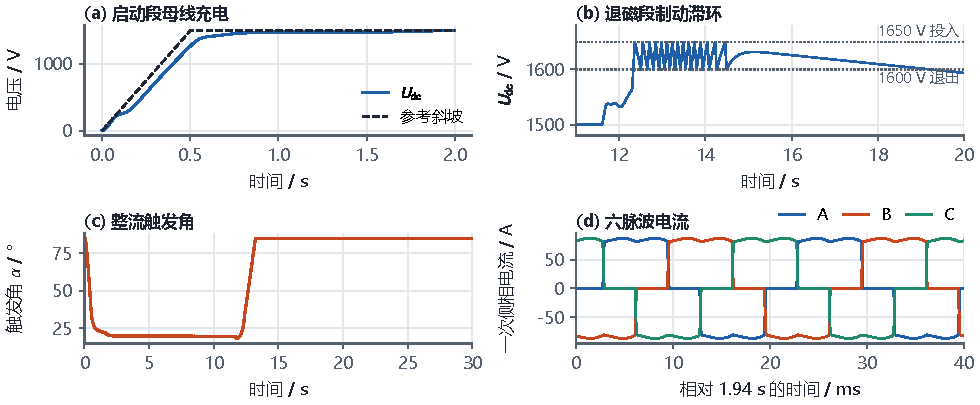
\includegraphics[width=\linewidth]{thyristor_interface}
\caption{晶闸管接口联合模型的运行结果（由保存的数据绘制）}
\label{fig:thy}
\end{figure}

该模型的全程能量流向见图~\ref{fig:joint-sankey}。按直流侧功率平衡方程核算，整流输出减去 H 桥输入、制动、泄放和电容储能变化后，全程残差 0.3797~kJ，相对整流输出为 0.00318\%。800 次换相的死区均为 2~$\mu$s，无同臂同时导通。步长由 2~$\mu$s 减为 1~$\mu$s 时，1.96--2~s 窗口的平均母线电压相差 0.017~V，平均电流相差 0.060~A，纹波由 251.21~A 降到 225.81~A。

\begin{figure}[htbp]
\centering
\begin{tikzpicture}[font=\footnotesize, >={Latex[length=1.6mm]},
  stage/.style={draw=#1, fill=#1!8, rounded corners=1.5pt, line width=0.6pt, align=center, minimum width=21mm, minimum height=12mm, inner sep=1pt},
  flow/.style={->, line width=0.8pt, color=black!70},
  sink/.style={draw=black!45, fill=rowtint, rounded corners=1.5pt, line width=0.5pt, align=center, minimum width=21mm, minimum height=8mm, font=\scriptsize, inner sep=1pt},
  drop/.style={->, line width=0.5pt, color=black!50}]
\node[stage=segbus] (g) at (0,0) {10~kV 母线送出\\\textbf{12.077~MJ}};
\node[stage=segrect] (r) at (3.2,0) {整流直流输出\\\textbf{11.936~MJ}};
\node[stage=seghb] (h) at (6.4,0) {H 桥直流输入\\\textbf{11.103~MJ}};
\node[stage=segpl] (c) at (9.6,0) {线圈侧输入\\\textbf{10.595~MJ}};
\node[stage=segpl] (p) at (12.8,0) {等离子体电阻\\\textbf{10.559~MJ}};
\draw[flow] (g)--(r);
\draw[flow] (r)--(h);
\draw[flow] (h)--(c);
\draw[flow] (c)--(p);
\node[sink] (a) at (0,-1.7) {变压器与桥损耗等\\0.141~MJ};
\node[sink] (b) at (3.2,-1.7) {制动 0.531~MJ\\泄放 0.071~MJ\\电容增量 0.230~MJ};
\node[sink] (d) at (6.4,-1.7) {H 桥器件损耗等\\0.508~MJ};
\node[sink] (e) at (9.6,-1.7) {$R\sub{cs}$ 等\\0.036~MJ};
\draw[drop] ($(g.east)+(0.25,0)$) |- (a.east);
\draw[drop] ($(r.east)+(0.25,0)$) |- (b.east);
\draw[drop] ($(h.east)+(0.25,0)$) |- (d.east);
\draw[drop] ($(c.east)+(0.25,0)$) |- (e.east);
\end{tikzpicture}
\caption{晶闸管接口模型 30~s 全程的能量流向。H 桥与线圈侧为代数累计，已扣除退磁回馈}
\label{fig:joint-sankey}
\end{figure}

两套模型由不同组员独立搭建，接口和母线电压都不相同，负载侧结果却高度一致（表~\ref{tab:compare}）：线圈侧能量相差 0.015\%，H 桥直流输入能量相差 0.03\%，1~$\mu$s 下的纹波相差 0.3\%。这说明负载和 H 桥的行为基本不受前级接口影响。差别集中在前级：晶闸管接口的交流侧送出能量多约 0.97~MJ，主要是制动消耗、母线电容留存和整流损耗，而双向接口把这部分回馈给了交流侧。

\begin{dtable}{htbp}{两种联合模型的对照}
\label{tab:compare}
\begin{tabularx}{\linewidth}{LRR}
\toprule
\headrow 项目 & 双向平均值接口 & 晶闸管整流接口 \\
\midrule
变压器与母线额定 & 10/1~kV，2200~V & 10/1.2~kV，1500~V \\
母线电容 & 20~mF & 0.2~F \\
退磁能量去向 & 回馈交流侧 & 电容与制动电阻 \\
母线电压范围 & 2187.0--2219.2~V & 最高 1650.14~V \\
功率级步长 & 1~$\mu$s & 2~$\mu$s（对比 1~$\mu$s） \\
平台段原边电流 & 10\,749.17~A & 10\,749.42~A \\
1~$\mu$s 电流纹波峰峰值 & 226.55~A & 225.81~A \\
交流侧累计能量 & 11.1059~MJ & 12.0770~MJ \\
H 桥直流输入累计能量 & 11.1059~MJ & 11.1030~MJ \\
线圈侧累计能量 & 10.5964~MJ & 10.5948~MJ \\
\bottomrule
\end{tabularx}
\end{dtable}

% !TEX root = ../main.tex

\chapter{跨环节分析}
\label{chap:analysis}

\section{各段的量级}

表~\ref{tab:segments} 把各段的额定值和主导动态放在一起：功率从 50~kW 跨到 59.6~MW，电流从 500~A 跨到 39.7~kA。联合模型的负载等级与实验四相同，平台段只有约 1~MW，所以交流母线几乎不受影响（电压 1.00005~pu）。联合仿真验证的是链路的拓扑、接口和控制配合，还不能代替对满功率工况的评估。

\begin{dtable}{htbp}{各段的额定值、时间常数与被控量}
\label{tab:segments}
\begin{tabularx}{\linewidth}{P{0.15\linewidth}P{0.25\linewidth}P{0.19\linewidth}P{0.13\linewidth}L}
\toprule
\headrow 环节 & 额定 & 主导时间常数 & 被控量 & 主要非理想性 \\
\midrule
\textcolor{segbus}{\textbf{10~kV 母线}} & 10~kV，短路容量 100~MVA & $\tau_Q=20$~ms，$\tau_E=50$~ms & 母线电压 & 电网阻抗压降 \\
\textcolor{segrect}{\textbf{CS 整流}} & 1.5~kV，39.7~kA，59.6~MW & $L\sub{eq}/R\sub{eq}=3$--$40$~s & 直流电压 & 换相重叠、300~Hz 纹波 \\
\textcolor{seghb}{\textbf{H 桥}} & 2200~V，500~A，50~kW & $L/R=100$~ms & 负载电流 & 死区、开关纹波 \\
\textcolor{segpl}{\textbf{等离子体}} & 100~V，10~kA，1~MW & $L_{\sigma,\mathrm{eq}}/R\sub{p}=12$--$17$~ms & 等离子体电流、磁链 & 回路纹波、磁链消耗 \\
\textbf{整机模型} & 2200~V 母线，约 1.13~MW & 同上 & 母线电压、$i\sub{p}$ & 上述各项的耦合 \\
\bottomrule
\end{tabularx}
\end{dtable}

\section{满功率工况下的母线能力}

实验一的整流器峰值 59.6~MW 能否接到实验二的母线上，是单独任何一个模型都无法回答的问题。

折算到交流侧：六脉波桥二次侧线电流有效值约 $0.816I_d=32.4$~kA，一次侧按变比折算为 3.89~kA，视在功率 67.4~MVA，略小于变压器额定 70~MVA。其中有功 59.6~MW，基波无功约 24~Mvar（对应 $\alpha\approx22^\circ$），基波视在功率 64.4~MVA，其余约 20~MVA 是 5、7、11 次等谐波形成的畸变功率。

短路比为
\begin{equation}
\mathrm{SCR}=\frac{S\sub{sc}}{P}=\frac{100}{59.6}=1.68,
\end{equation}
低于通常作为弱交流系统分界的 3\cite{ieee1204}。沿用第 \ref{chap:bus} 章的相量关系，维持母线 1.0~pu、负载 59.6~MW 和基波无功 24~Mvar 时，以 $S\sub{sc}$ 为基准有
\begin{equation}
E\sub{req}=\Bigl|V+\frac{P-\mathrm{j}Q}{V}\,z_g\Bigr|=1.455\ \mathrm{pu},
\end{equation}
远超 1.15~pu 的限幅。降低母线电压并不能缓解：$V$ 由 1.0~pu 降到 0.8~pu，$E\sub{req}$ 只由 1.455~pu 降到 1.411~pu，因为电压越低电流越大。即使把无功完全补偿，$E\sub{req}$ 仍为 1.261~pu。

结论是这条 100~MVA 母线送不出 59.6~MW，限制来自短路容量而不是控制器。图~\ref{fig:scr}(a) 和表~\ref{tab:scr} 给出 $E\sub{req}$ 随短路容量的变化：约 270~MVA 时 $E\sub{req}$ 降到 1.15~pu，取 300~MVA（SCR $\approx5$）时为 1.132~pu。这一结果与实验二自身的重载工况一致：19.3~MW 时 $E$ 已顶到 1.15~pu，母线掉到 0.879~pu。真实装置中，CS 整流器需要接到短路容量更大的母线上，或配置无功补偿和调压手段。

\begin{figure}[htbp]
\centering
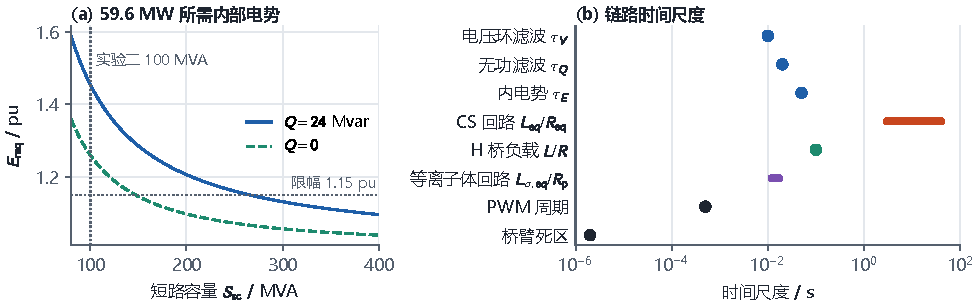
\includegraphics[width=\linewidth]{analysis_scr_time}
\caption{(a) 维持 59.6~MW 所需内部电势随短路容量的变化，(b) 链路各环节的时间尺度，颜色对应图~\ref{fig:chain} 的环节}
\label{fig:scr}
\end{figure}

\begin{dtable}{htbp}{短路容量与维持 59.6~MW 所需的内部电势}
\label{tab:scr}
\begin{tabularx}{\linewidth}{LRRRRR}
\toprule
\headrow $S\sub{sc}$ / MVA & 100 & 200 & 250 & 300 & 350 \\
\midrule
SCR & 1.7 & 3.4 & 4.2 & 5.0 & 5.9 \\
$E\sub{req}$ / pu & 1.455 & 1.206 & 1.161 & 1.132 & 1.111 \\
\bottomrule
\end{tabularx}
\end{dtable}

\section{时间尺度}

图~\ref{fig:scr}(b) 展示了链路的时间尺度：从 2~$\mu$s 的死区到 40~s 的 CS 回路，跨越七个数量级。同样 10~kA 的电流，在 CS 回路和等离子体回路中的时间常数相差约三个数量级。

这一跨度决定了建模策略。用 2~$\mu$s 步长跑完实验一的 460~s 需要 $2.3\times10^8$ 步，是联合模型 30~s 工况的 15 倍；反过来用 0.01~s 步长则完全无法分辨死区。因此分段模型和联合模型各有用途：平均值模型用于长时间磁体过程，开关级模型用于控制与能量校核，联合模型只覆盖等离子体负载的 30~s 放电周期。

\section{“指令—实际”偏差的比较}

四段都存在指令与实际的偏差，性质却各不相同（表~\ref{tab:losses}）。母线 1.2\% 的下降是下垂设计的目标，由 PI 在慢时间尺度上跟随；死区 0.8\% 的损失每个开关周期都出现，只能由积分器在几十毫秒尺度上平均掉；整流 0.46\% 的压降由负载电流和变压器漏抗决定，改控制参数无法消除；约 2.3\% 的电流纹波则是电流波形本身的组成部分，只能通过提高开关频率或加大回路电感减小。按性质区分，才能判断哪些偏差值得补偿。

\begin{dtable}{htbp}{四段的“指令—实际”偏差}
\label{tab:losses}
\begin{tabularx}{\linewidth}{P{0.12\linewidth}P{0.2\linewidth}P{0.27\linewidth}L}
\toprule
\headrow 环节 & 偏差来源 & 相对量级 & 处理方式 \\
\midrule
10~kV 母线 & 下垂与电网阻抗压降 & 1.2\%（2.44~MW 工况） & 下垂控制加 PI 抬高 $E$ \\
CS 整流 & 换相重叠、离散采样 & 0.46\%（6.9~V / 1500~V） & 闭环调节触发角 \\
H 桥 & 2~$\mu$s 死区 & 0.80\%（17.6~V / 2200~V） & 积分器补偿或电流方向前馈 \\
等离子体 & 回路电流纹波 & 约 2.3\%（227~A / 10~kA） & 提高开关频率或加大回路电感 \\
\bottomrule
\end{tabularx}
\end{dtable}

\section{模型的适用边界}

\begin{itemize}
  \item 联合模型只运行在约 1~MW 负载下，没有覆盖实验一的 59.6~MW 工况；上文的母线能力核算是相量关系下的静态结论，不能回答满功率接入时的暂态过程。
  \item 整机的双向平均值接口是建模假设：理想同步、变比和 20~mF 缓冲电容都不是课堂给定，也不代表已设计好的整流器。实验一的 CS 工况是独立的 1.5~kV、460~s 对照，并未接入整机。
  \item 实验四教程提到的 \texttt{Power\_div\_R}、\texttt{Resistive\_feedforward}、\texttt{LP\_EXTRA} 等功率控制接口未完整保留，当前版本使用电流给定斜坡及 $R\sub{p}i\sub{ref}$ 前馈。
  \item 器件模型为分段线性，不含开关暂态、反向恢复和结温；实验二的测试变压器已理想化；等离子体负载是单端口降阶模型，不含空间耦合、真空室涡流和失超保护。
  \item 整流器 PI、H 桥 $K_p$ 和退磁 $k_\psi$ 只取了一组设计值，尚未做参数敏感性分析。
  \item 实验四的整机参考波形约为 100~MW，缺少完整参数和原始数据；本模型只有 10~kA、1~MW，两者只能比较形状和时序，不能据此宣称达到该功率等级。
\end{itemize}

% !TEX root = ../main.tex

\chapter{结论与展望}
\label{chap:conclusion}

本报告整合了课程的仿真工作，按功率流向完成了从 10~kV 交流母线到等离子体负载的建模与校核，并把各环节接入了同一电气网络。主要结论如下。

\begin{enumerate}
  \item \textbf{10~kV 母线。}六个工况全部通过相量校核，默认工况母线 0.987803~pu、内部电势 1.017047~pu；重载工况在 0.110525~s 触及 1.15~pu 上限，积分状态被冻结，母线停在 0.878646~pu。
  \item \textbf{CS 整流供电。}460~s 全过程电流峰值 39.746~kA、输入功率峰值 59.619~MW、磁场 11.482~T、储能 0.7571~GJ，八个关键时刻的电流与 ODE 基准最大相差 0.247\%；六脉波详细模型验证了 300~Hz 纹波和触发顺序。
  \item \textbf{H 桥电流环。}五段给定稳态误差 0.68--1.77~A，载波 2000.0~Hz；修正死区实现后，两桥臂各 1592 次换相的间隔全部为 2~$\mu$s，无桥臂直通；调制律偏差与死区损失 17.60~V 相符，负载回路方程稳态残差均方根 2.85~V。
  \item \textbf{可变等离子体负载。}平台段约 10~kA、1~MW，磁链两条独立路径的最大残差约 0.011~Wb；线圈侧多出的功率由励磁储能增长和原边电阻损耗解释；1~$\mu$s 下电流纹波约 2.3\%，而 10~$\mu$s 步长会明显放大纹波，并使退磁尾段失去窄脉冲。
  \item \textbf{全链路联合。}整机模型连续运行 30~s，平台段母线 2199.98~V、等离子体电流 9999.28~A，门极窗口实测 2~$\mu$s 死区，退磁向交流侧净回馈 0.559~MJ。晶闸管接口的对照模型全程直流能量相对残差 0.00318\%，退磁能量由电容和制动支路吸收。两套独立模型的线圈侧能量相差 0.015\%。
  \item \textbf{接口分析。}100~MVA 母线无法支撑实验一的 59.6~MW 峰值负载，所需内部电势 1.455~pu 超出 1.15~pu 限幅，短路容量需提高到约 270~MVA 以上。
\end{enumerate}

后续工作可以沿三个方向展开：一是把联合模型的负载提升到实验一的功率等级，并按第 \ref{chap:analysis} 章的结果配置短路容量和无功补偿，观察脉冲负载对母线的暂态影响；二是对整流器 PI、电流环参数和退磁系数 $k_\psi$ 做敏感性分析；三是把等离子体负载由单端口模型扩展为带空间耦合的降阶模型，使磁链预算更接近真实放电。

% !TEX root = ../main.tex
\chapter{项目协作与公开发布}
\label{chap:workflow}
本项目由六位贡献者共同完成，公开成果位于 \url{\repourl}。模型采用 MATLAB R2026a；功能修改在分支中完成，再根据验证结果合并。技术正文保留原报告的分析与结论，公开版本调整身份信息、封面和文件导航。
\section{贡献者}
贡献者按公开 GitHub 用户名署名：\texttt{Hale-debug}、\texttt{Jerry131131}、\texttt{KiloxGo}、\texttt{qikexiu4K4}、\texttt{southever}、\texttt{zhyz18zsw060620}。此名单按账号排序，不表示贡献大小。公开版本不保留历史提交身份和私人邮箱。
\section{成果组织}
\texttt{Project/Models} 保存联合模型与独立模块，\texttt{Project/Variants} 保存修正版和对比变体，\texttt{Project/Scripts} 保存运行与导出脚本，\texttt{Project/Materials} 保存数值表格、波形及模型视图。\texttt{docs/} 说明架构、假设、验证与数据口径，\texttt{report/} 保存本报告及公开版源码。
\section{验证范围}
报告包含整机联合仿真与历史对照分析。公开仓库的实际可复现范围以附录和仓库文档为准；未分发的历史对照实现不应描述为已经在当前公开版本中重跑。协作记录和原始教学资料不随公开快照分发。


\FloatBarrier
\printbibliography[heading=bibintoc]

\appendix
\captionsetup{list=no}
% !TEX root = ../main.tex

\chapter{模型主要参数}
\label{app:params}

\newcommand{\paramtable}[2]{%
\begin{dtable}{H}{#1}
\begin{tabularx}{\linewidth}{P{0.28\linewidth}P{0.3\linewidth}L}
\toprule
\headrow 参数 & 取值 & 说明 \\
\midrule
#2
\bottomrule
\end{tabularx}
\end{dtable}}

\paramtable{10~kV 母线与电网等值}{%
基准 $V_b$，$S_b$ & 10~kV，10~MVA & 线电压有效值；$S_b$ 仅用于标幺化 \\
短路容量，$X/R$ & 100~MVA，5 & $R_g=0.196116\ \Omega$，$L_g=3.121285$~mH \\
下垂系数 & 0.05 & $v\sub{ref}=1-0.05q\sub{f}$ \\
PI & $K_p=0.5$，$K_i=10\ \mathrm{s^{-1}}$ & $E\in[0.85,1.15]$~pu \\
一阶环节 & $\tau_V=10$，$\tau_Q=20$，$\tau_E=50$~ms & 初值 1、0、1 \\
测试变压器 & 10~MVA，Yg/Yg，10:1 & 漏抗、励磁、饱和关闭 \\
默认负载 & $R_2=X_2=0.2\ \Omega$ & 折算一次侧 $20+\mathrm{j}20\ \Omega$ \\
}

\paramtable{CS 整流供电}{%
变压器 & 70~MVA，10/1.2~kV，$\Delta$/Y & 绕组电阻 0.005~pu，漏抗 0.05~pu \\
直流参考 & 1500~V & 初始触发角 $22.192^\circ$ \\
触发角范围 & $5^\circ$--$80^\circ$ & PI 输出限幅 \\
负载 & $R\sub{eq}$、$L\sub{eq}$ 九个关键点 & PCHIP 插值，0.01~s 网格 \\
平均值模型 & ode15s，最大步长 0.01~s & 0--460~s \\
详细模型 & 离散，50~$\mu$s & 0--0.5~s \\
}

\paramtable{H 桥电流环}{%
直流母线 & 2200~V & 受控电压源，负极接地 \\
器件 & $R\sub{on}=20\ \mu\Omega$，$V_f=2$~V & IGBT 与反并联二极管 \\
负载 & $R=0.2\ \Omega$，$L=20$~mH & 初始电流 0 \\
电流环 & $K_p=12.56637$，$K_iT_c=6.2832\times10^{-3}$ & 电压限幅 $\pm400$~V，$m\sub{H}$ 限幅 $\pm0.95$ \\
采样与调制 & 50~$\mu$s 保持 + 50~$\mu$s 延迟 & 载波 2~kHz，死区 2~$\mu$s \\
仿真 & 定步长 1~$\mu$s，0--0.42~s & 局部后向欧拉 \\
}

\paramtable{可变等离子体负载}{%
互感 & $L_1=L_2=1$~H，$k=0.99999$ & 原边串联 $R\sub{cs}=20\ \mu\Omega$ \\
$R\sub{p}$ 查表 & 15、10、100 000 m$\Omega$ & 断点 0.6、1.6、11.6、12.1、12.3~s \\
$L\sub{p}$ 查表 & 150、100~$\mu$H & 断点 0.6、1.6~s \\
并联电阻 & 两支 100~k$\Omega$ & 分别跨 $L\sub{p}$、$R\sub{p}$ \\
电流环 & $K_p=0.1$~V/A，$K_i=6.25$~V/(A$\cdot$s) & 前馈 $R\sub{p}i\sub{ref}$，限幅 $\pm400$~V \\
退磁 & $k_\psi=2$~V/Wb & 12.3~s 起接替，限幅 $\pm400$~V \\
仿真 & 定步长 10~$\mu$s，0--30~s，载波 4~kHz & 基线模型 \\
}

\paramtable{整机模型新增参数}{%
变压器 & 10/1~kV & 继承实验二模型 \\
AC/DC 接口 & 双向平均值，$r=2.2$ & 理想同步参考，属建模假设 \\
直流缓冲电容 & 20~mF，预充 2200~V & 属建模假设 \\
PWM 与死区 & 2~kHz，2~$\mu$s & 沿用实验三，修正版死区 \\
求解器 & ode3，固定步长 1~$\mu$s & 局部后向欧拉，每步 3 次迭代 \\
记录 & 综合信号 10~$\mu$s，门极 1~$\mu$s & 能量按 1~$\mu$s 积分 \\
}

\paramtable{晶闸管接口对照模型的参数}{%
变压器接法 & 70~MVA，10/1.2~kV，副边浮置 Y & 直流负极接地 \\
平波电抗、电阻 & 5~mH，0.02~$\Omega$ & 平滑整流电流 \\
母线电容 & 0.2~F & 缓冲脉冲功率 \\
电压环 & $K_p=0.03$，$K_i=0.5$ & 输出为触发角，范围 $5^\circ$--$85^\circ$ \\
电流阻尼、启动斜坡 & 0.01 $^\circ$/A，3000~V/s & 抑制充电过冲 \\
晶闸管 & 1 m$\Omega$，0.8~V & 分段线性模型 \\
制动 & 5~$\Omega$，1650~V 投入，1600~V 退出 & 吸收退磁能量 \\
泄放电阻 & 1000~$\Omega$ & 并联母线 \\
仿真 & 定步长 2~$\mu$s，0--30~s & 电流环采样 50~$\mu$s \\
}

% !TEX root = ../main.tex
\chapter{公开版复现方法}
\label{app:repro}
\sloppy
公开模型需要 MATLAB/Simulink R2026a、Simscape 与 Simscape Electrical。整机采用 accelerator 模式，还需可用的本机编译器。请在仓库根目录执行：
\begin{codeblock}[language=Matlab]
addpath('Project')
start_project
run_integrated('startup')
export_integrated_materials('startup')
run_integrated('full')
export_integrated_materials('full')
verify_hbridge_deadtime
run_baselines
export_writing_materials
run_pwm_study
export_pwm_study
\end{codeblock}
\texttt{run\_baselines} 依次运行下垂电源、原 H 桥、可变负载及 460~s CS 平均值模型。原始 MAT 生成于 \texttt{Project/Results/raw}，不随 Git 分发。PNG、PDF 和 CSV 可直接读取；可编辑 FIG 由导出脚本生成。
\section{历史对照的可用范围}
正文保留原报告的母线六工况、ODE 基准和晶闸管接口联合模型的对照分析及数值。当前公开快照不分发全部历史实现，尤其不包含另一套晶闸管接口联合模型；因此相应结果作为报告中的历史对照材料，不宣称可以仅用本快照重新计算。当前整机采用双向平均值 AC/DC，具体边界见仓库的模型假设说明。
\section{主要模型}
\begin{dtable}{H}{公开版模型文件}
\begin{tabularx}{\linewidth}{P{0.62\linewidth}L}
\toprule
\headrow 路径 & 内容 \\
\midrule
\texttt{Project/Models/tokamak\_integrated.slx} & 整机联合模型 \\
\texttt{Project/Models/cs\_rectifier\_average.slx} & 独立 460~s CS 模型 \\
\texttt{Project/Models/droop\_source.slx} & 下垂电源模型 \\
\texttt{Project/Models/hbridge\_rl.slx} & 原 H 桥基线 \\
\texttt{Project/Models/plasma\_load.slx} & 独立可变负载 \\
\texttt{Project/Variants/hbridge\_rl\_verified.slx} & H 桥死区修正版 \\
\texttt{Project/Variants/plasma\_2khz\_detail.slx} & PWM 敏感性变体 \\
\bottomrule
\end{tabularx}
\end{dtable}
报告使用 CTEX、XeLaTeX 与 biber 编译，入口为 \texttt{report/source/main.tex}。从该目录执行 \texttt{latexmk -xelatex main.tex}。报告分析图保留为既有导出文件；联合模型与模块图表可使用公开脚本重新生成。


\end{document}
